%%%%%%%%%%%%%%%%%%%%%%%%%%%%%%%%%%%%%%%%%%%%%%%%%%%%%%%%%
%%%%%IMPORTS:

%packages a utilizar:
\documentclass{report}
\usepackage[T1]{fontenc}     % Fontes T1
\usepackage[utf8]{inputenc}  % Input UTF8
\usepackage[top=3cm,bottom=3cm,left=3cm,right=2.5cm,asymmetric]{geometry} %fronteiras
%\usepackage[nottoc]{tocbibind}
\usepackage[table]{xcolor} %Colorir tabelas
\usepackage[backend=biber, style=ieee]{biblatex} %bibliografia
\usepackage{csquotes}  % referências
\usepackage[portuguese]{babel} %Usar língua portuguesa
\usepackage{blindtext} 
\usepackage[printonlyused]{acronym}  %Acrónimos
\usepackage{hyperref}  %Autoref no índice
\usepackage{graphicx}  %Usar imagens
\usepackage{titling}
\usepackage{multicol} %multicoluna de texto
\usepackage{adjustbox}
\renewcommand{\figurename}{Fig.} 
\renewcommand{\tablename}{Tabela} 
\usepackage[font=small,tableposition=top]{caption} 
\usepackage[font=small]{subcaption}
\usepackage{xcolor} %cor nos textos
\usepackage{amsmath} %matematica
\usepackage{amssymb} %simbolos matematicos
\graphicspath{ {./images/} } %directorio das imagens
\usepackage{fancyhdr}
\usepackage{authblk}
\usepackage{float} %Posicionamento exacto das figuras no texto
\usepackage{url}   %referencias URL
\usepackage{blindtext}
\def\UrlBreaks{\do\/\do-} %não cortar referencias

\usepackage{indentfirst} %Garantir avanço do primeiro parágrafo
\hypersetup{pdfborder=0 0 0} %Remover a caixa vermelha das referências
\usepackage{chngcntr} %Numeração contínua das figuras
\counterwithout{figure}{chapter} %Numeração contínua de figuras
\counterwithout{table}{chapter} %Numeração contínnua de tabelas
\setlength{\parskip}{0.2cm} %Aumento de espaçamento entre parágrafos

\usepackage{hyperref}

 
\begin{document}	
	%Definições do Relatório

%Dados Gerais:
\def\titulo{Projecto Final: \\ Máquina de Lavagem de Roupa}
\def\data{Junho de 2022}
\def\versao{Ver.: 1.13}
\def\departamento{Departamento de Electrónica Telecomunicações e Informática}
\def\empresa{Universidade de Aveiro}
\def\logotipo{logotipo_ua.png}

%Dados dos Autores:
%primeiro autor:
\def\pautor{João Pedro Nunes Vieira} 
\def\numpautor{Nº Mec.:  50458}
\def\contactopautor{joaopvieira@ua.pt}
%segundo autor:
\def\sautor{Leandro Roque Costa} 
\def\numsautor{Nº Mec.: 110326}
\def\contactosautor{lrc@ua.pt}
%
\def\autores{\pautor \\ \sautor}

	%Capa do Relatório:
\begin{titlepage} 
	\begin{center}
	\includegraphics[scale=0.50]{\logotipo}
	\line(1,0){350} \\ 
		\vspace*{2mm}
	{\Large \uc} \\
		\vspace*{2mm} 	
	{\Huge \titulo} \\
		\vspace*{2mm}
	\line(1,0){350} \\ 
		\vspace*{2mm}
	{\Large \empresa} \\
		\vspace*{20mm}
	{\Large \autores} \\ 
		\vspace*{\fill}
	\end{center}

	\begin{flushright} 
		{\large \departamento} \\ 
		{\versao} 
	\end{flushright}

\end{titlepage}

	%Página de Título:
\predate{\begin{flushright}\small}
\postdate{\par\end{flushright}}

\title{ 
	{\huge\textbf{\titulo} } \\ 
	{\large \departamento\\ \empresa} }

\author{

    \begin{tabular}{l}
        \pautor, \numpautor\hfil \\
        \contactopautor
    \end{tabular}
    \and
    \begin{tabular}{l}
        \sautor, \numsautor\hfil \\
        \contactosautor
    \end{tabular}
    \and
    \begin{tabular}{l}
        \tautor, \numtautor\hfil \\
        \contactotautor
    \end{tabular}
    \and
    \begin{tabular}{l}
        \qautor, \numqautor\hfil \\
        \contactoqautor
    \end{tabular}
}




\date{\vspace{\fill}{\data}} 
\maketitle
	\begin{abstract}

O presente relatório aborda a comunicação entre aplicações seguindo um modelo Cliente-Servidor, usando conceitos abordados no decorrer da Unidade Curricular de Laboratórios de Informática, nomeadamente programação de sockets TCP, Criptografia, Documentação JSON, programação em Python, etc... \\
Este trabalho é relevante pois com o avanço tecnológico actual, a aprendizagem dos conceitos anteriormente referidos torna-se imperativa para os estudantes de cursos ligados à tecnologia de informação.\\
O projecto foi realizado por duas pessoas, tendo como objectivo o desenvolvimento das capacidades de trabalho em grupo, desenvolvimento e estruturação de código, realização de testes funcionais e planeamento através da plataforma \textbf{code.ua.pt}. \\
Foi possível implementar com sucesso um modelo de comunicação entre aplicações Cliente-Servidor em gênero "Jogo High-Low" com funcionalidade de segurança(encriptação) de forma simples, prática e eficaz, conseguindo-se corrigir todos os erros encontrados.

\end{abstract}
	
%%%%%%%%%%%%%%%%%%%%%%%%%%%%%%%%%%%%%%%%%%%%%%%%%%%%%%%%%
%%%%%INDICE:

\renewcommand{\contentsname}{Índice}
\tableofcontents
\listoffigures
\pagenumbering{roman}

%%%%%%%%%%%%%%%%%%%%%%%%%%%%%%%%%%%%%%%%%%%%%%%%%%%%%%%%%
%%%%%ACRÓNIMOS:

\chapter*{Acrónimos}
\begin{acronym}

\acro{ua}[UA]{Universidade de Aveiro}
\acro{miect}[MIECT]{Mestrado Integrado em Engenharia de Computadores e Telemática}
\acro{uc}[UC]{Unidade Curricular}
\acro{labi}[LABI]{Laboratórios de Informática}
\acro{codeua}[CodeUA]{code.ua.pt}
\acro{afinet}[AF\_INET]{Address Family INET}
\acro{ipv4}[IPv4]{Internet Protocol version 4}
\acro{str}[SOCKET\_STREAM]{Stream Sockets}
\acro{tcp}[TCP]{Transmission Control Protocol}
\acro{aes-128}[AES-128]{Advanced Encryption Standard - 128 bits key}
\acro{ecb}[ECB]{Electronic CodeBook}
\acro{iana}[IANA]{Internet Assigned Numbers Authority}
\acro{utf-8}[UTF-8]{8-bit Unicode Transformation Format}
\acro{json}[JSON]{JavaScript Object Notation}

\end{acronym}

%%%%%%%%%%%%%%%%%%%%%%%%%%%%%%%%%%%%%%%%%%%%%%%%%%%%%%%%%
%%%%%HEADERS & FOOTERS:

\pagestyle{fancy}
\fancyhf{}
\rhead{\titulo}
\lhead{Introdução}
\cfoot{\thepage}

%%%%%%%%%%%%%%%%%%%%%%%%%%%%%%%%%%%%%%%%%%%%%%%%%%%%%%%%%
%%%%%INTRODUÇÃO:

\chapter{Introdução}
\label{chap.Intro}
\pagenumbering{arabic}
\begin{multicols}{2}

Devido ao grande avanço tecnológico das últimas décadas, a internet tornou-se uma ferramenta essencial para o funcionamento da sociedade. Sendo a internet um sistema global de redes de computadores interligados entre si usando um conjunto próprio de protocolos, torna-se fundamental o estudo da comunicação entre aplicações, já que esta é a base fundamental da web. \\

Assim, no decorrer do segundo semestre no âmbito da \ac{uc} de \ac{labi} do \ac{miect}, realizou-se este trabalho com o objetivo de aprender e aprofundar o estudo de diversos temas, nomeadamente a programação em Python, criptografia, depuração, comunicação entre aplicações e documentos tipo CSV e JSON. \\ 

O presente trabalho surge no tema de desenvolvimento de uma aplicação Cliente que tenta adivinhar um número inteiro aleatório secreto (entre 0 e 100) gerado por um Servidor, usando protocolos e sockets API numa rede de computador. \\ 

Ao longo deste relatório será indicado e descrito o processo de implementação das aplicações, da sua protecção e segurança, os testes efectuados de modo a garantir o funcionamento pretendido e a análise de resultados obtidos.

\end{multicols}

\section{Ferramentas}
\label{sec.ferramentas}
No desenvolvimento deste trabalho foram utilizadas algumas ferramentas e conhecimentos teóricos e práticos abordados no decorrer da \acf{uc}, \ac{labi}:

\begin{itemize}
	\item \textsl{Sistema Operativo Linux:} Ubunto Ver.20.04  
	\item \textsl{Editor de texto Geany:} Editor de texto que suporta a linguagem de programação Python3 que irá ser usada para a elaboração deste trabalhjo.
	\item \textsl{Ficheiros Python:} Fornecidos pelos docentes da \ac{uc} para inicialização do trabalho. 
\end{itemize}

\clearpage

\section{Regras}
\label{sec.regras}
A aplicação Servidor–Cliente rege-se pelas seguintes normas: \\

O Servidor aceita vários Clientes simultaneamente desde que não tenham IDs iguais. Se um Cliente entrar com um ID igual a outro que esteja actualmente a jogar o Servidor deve negar o pedido de conexão. \\

Se a conexão for aceite, o Servidor deve gerar um número inteiro aleatório, entre 0 e 100, para o usuário adivinhar e também um número aleatório de tentativas, entre 10 e 30, que tem para o fazer. \\

O Servidor deve criar e actualizar um ficheiro de tipo csv que regista os resultados dos diversos Clientes quando estes terminam o jogo correctamente. O usuário pode terminar o jogo normalmente quando acerta no número (nesse caso o Servidor deve registar o jogo como sucesso) ou por esgotamento de tentativas (o jogo deve ser registado como fracasso). \\

Além disso, o usuário pode desistir do jogo a qualquer momento com a operação \textit{quit} (o Servidor regista o jogo como desistência). Sempre que o Cliente faz um pedido de operação ao Servidor deve receber alguma notificação a indicar se foi aceite ou não. \\

\textit{Nota: Decidiu-se fazer algumas alterações ao trabalho proposto de forma a explorar as possibilidades das ferramentas usadas. Nomeadamente, implementou-se a hipótese de o usuário mudar o seu ID quando recebe uma notificação do Servidor a indicar que o seu ID é igual a um já existente e, para além disso, também se adicionou no fim do jogo a possibilidade de o usuário jogar novamente caso assim queira.} \\

%%%%%%%%%%%%%%%%%%%%%%%%%%%%%%%%%%%%%%%%%%%%%%%%%%%%%%%%%
%%%%%CAPÍTULO 1: Implementação

\chapter{Implementação}	
\label{chap.aplicações}
\lhead{Comunicação entre Aplicações}
A comunicação entre aplicações é o tema principal deste trabalho, tendo como objetivo a implementação de uma aplicação-Servidor e uma aplicação-Cliente que comunicam entre si para executar o jogo de estilo \textit{High-Low}, tal como descrito na Introdução \ref{chap.Intro}. Esta comunicação é feita através de programação de sockets e o Servidor comunica com vários Clientes simultaneamente. \\

Tanto a aplicação-Cliente como a aplicação-Servidor são iniciadas usando uma interface de linha de comandos (Consola/terminal Linux ou Linha de Comandos CMD Microsoft) e invocando os comandos:
\begin{center}
\Large\textsl{"python3 client.py client\_id porta endereço"} 
\Large\textsl{"python3 server.py porta"} 
\end{center}
Por exemplo, um Cliente com client\_id "João" conecta-se ao Servidor de porto 1234 com endereço 127.0.0.1 como ilustrado na figura \ref{fig:conexão-bem-executada1}. \\ 

	\begin{figure}[H]
		\centering
		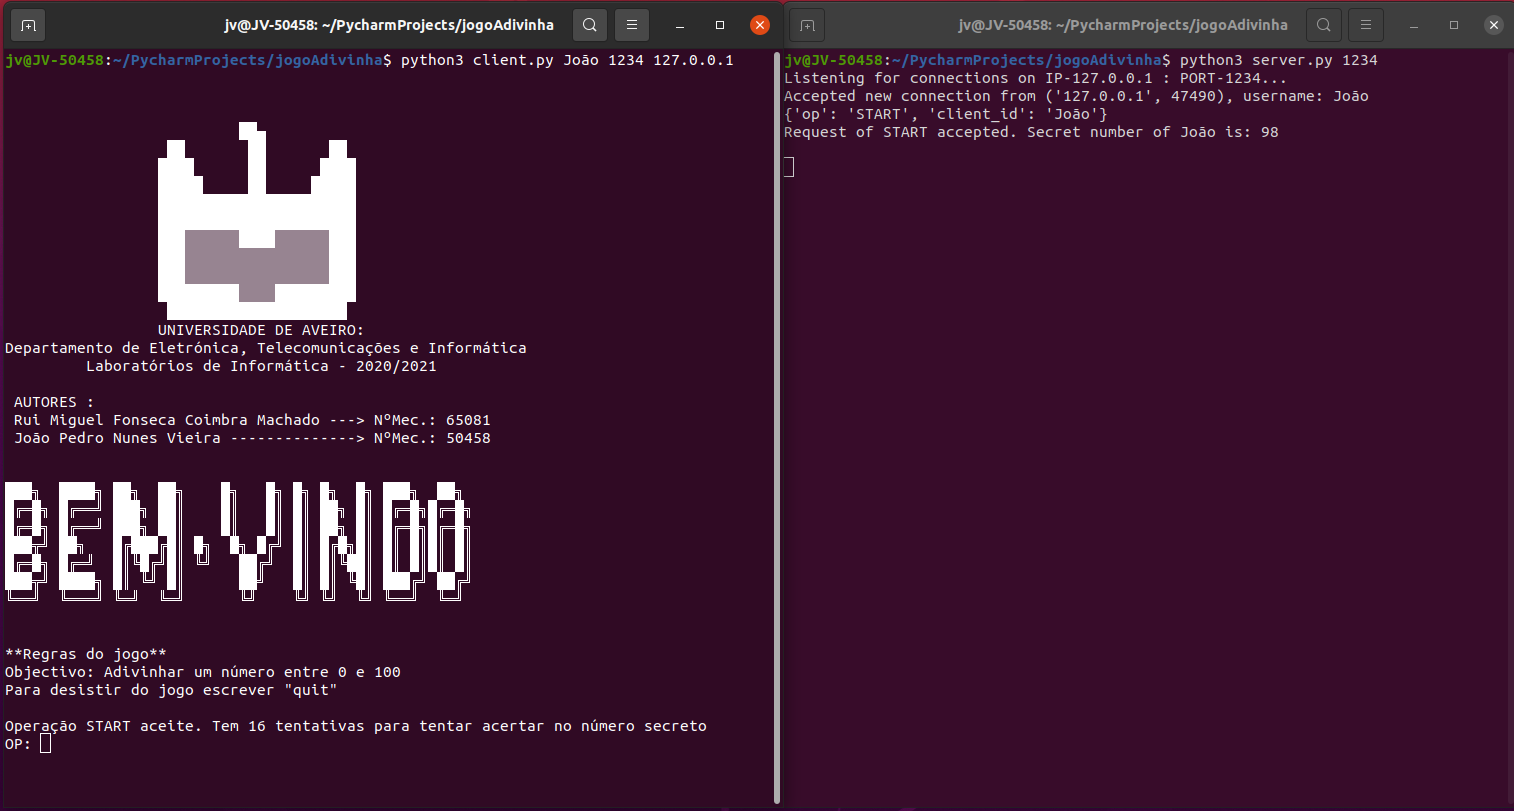
\includegraphics[width=12cm]{conexão-bem-executada}
		\caption{Exemplo de conexão de um Cliente ao Servidor.\\}
		\label{fig:conexão-bem-executada1}
		\flushleft\small\textit{O porto do servidor é definida pelo Servidor na sua iniciação, sendo o seu endereço pré-definido.}
	\end{figure} 

\newpage
O usuário deve introduzir um identificador pessoal (client\_id) que ainda não tenha sido escolhido por outro, como será demonstrado no capitulo \ref{chap.testes e resultados} \\
Uma vez aceite a conexão pelo Servidor, é fornecido ao Cliente um número máximo de tentativas para adivinhar o número secreto. Tanto o número secreto como o número máximo de tentativas são gerados aleatoriamente pelo Servidor, sendo atribuídos números diferentes a cada Cliente.
Sempre que o usuário tenta adivinhar o número tanto o Servidor como o Cliente registam essa tentativa e o Servidor informa o usuário se o número introduzido é inferior (\textit{smaller}) ou superior (\textit{larger}) ao número secreto. O usuário pode então voltar a introduzir outro número tentando acertar no número secreto. O jogo acaba caso o usuário acerte no número secreto, recebendo a mensagem \textit{equals}, ou caso esgote o seu número de tentativas, sendo lhe dada a opção de jogar novamente. Além disso, o usuário pode desistir a qualquer momento através da operação \textit{quit}.\\
%%%%%
\section{Socket}
\label{sec.socket}
Tanto o Cliente como o Servidor devem ter sockets de conexão estruturados com a mesma família, tipo e nome/interface. \\
A comunicação entre as aplicações é feita de forma local ou remota, sendo que, para este efeito, foram implementados sockets com protocolo de rede da familia \ac{afinet} (apenas suporta \ac{ipv4}) de tipo \ac{str} (orientado à ligação) com um protocolo de transmição \ac{tcp}.

\subsubsection{Aplicação-Servidor}
A base deste trabalho é a programação entre Sockets TCP.
O código da aplicação-Servidor começa por criar uma socket da família IPV4 do tipo TCP com a instrução socket. Seguidamente, dá-se um nome ao socket com a instrução bind, nome esse que é composto por um endereço (IPv4 e porto) para os Clientes poderem estabelecer uma conexão. Finalmente, coloca-se o socket à escuta com o comando listen() para que esteja disponível para conexões. Além disso, chama-se a função create\_file que cria um ficheiro do tipo csv para registar os resultados dos Clientes. O nome do ficheiro a ser criado é declarado no cabeçalho do código com uma variável global, a função create\_file, e antes de criar um ficheiro certifica-se que não existe nenhum ficheiro com o mesmo nome no directório actual, só então cria um ficheiro novo.

\begin{figure}[H]
	\centering
	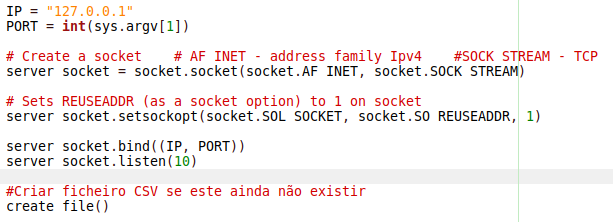
\includegraphics[width=10cm]{server1}
	\caption{Código inicial do Servidor.\\}
	\label{fig:server1}
\end{figure} 

\clearpage

Para que um Servidor possa atender vários Clientes ele necessita de ter uma lista para armazenar os sockets associados aos Clientes ativos. Essa lista é a lista clients[] declarada no cabeçalho do programa. Além dessa lista criou-se também uma lista nicknames[] com os IDs dos Clientes para o Servidor poder imprimir mensagens internas e ser mais fácil de o monitorizar.
O método select permite ficar à escuta de informação de múltiplas fontes, indicando depois qual das fontes possui informação a ser consumida. Este método é usado neste trabalho apenas para ver que Clientes enviaram mensagens.

Sempre que um Cliente novo se conecta ao Servidor, este é adicionado à lista clients[] e é lhe criado um endereço particular para que o Servidor consiga enviar mensagens só para ele. Além disso, o Cliente está programado para enviar automaticamente o seu ID, assim o Servidor recebe esse ID e adiciona-o à lista nicknames[]. A partir desse momento todas as mensagens internas imprimidas no Servidor usam esse ID de forma a facilitar a compreensão do Servidor

\begin{figure}[H]
	\centering
	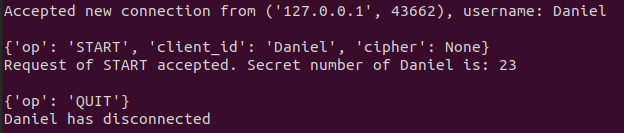
\includegraphics[width=10cm]{nickname}
	\caption{Utilização da lista nicknames[] para impressão de mensagens internas.\\}
	\label{fig:nickname}
\end{figure} 

Sempre que um Cliente com conexão já estabelecida envia uma mensagem é invocada a função new\_msg(), que lida com as mensagens.
Se um Cliente terminar o programa por alguma razão, o Servidor elimina-o das listas clients[] e nicknames[] e também do dicionário gamers[], que iremos falar mais à frente. Também fecha o endereço criado para esse Servidor.
 
\begin{figure}[H]
	\centering
	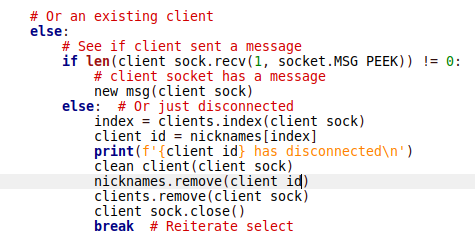
\includegraphics[width=10cm]{disconect}
	\caption{Cliente envia mensagem\\}
	\label{fig:disconect}
\end{figure} 

Como dito anteriormente, a função new\_msg() lida com as mensagens. Esta foi implementada para apenas lidar com mensagens dicionário no formato esperado (primeira chave do dicionário deve ser "op"). A função verifica a operação enviada pelo Cliente e, de acordo com a operação encontrada, encaminha o programa para as funções pretendidas. As opções de operação são: Start, Guess, Quit e Stop. Se receber uma mensagem no formato esperado, mas com uma operação fora das opções estabelecidas, retorna ao Cliente uma mensagem de erro.
Inicialmente adicionou-se uma linha de código que imprime as mensagens recebidas do Servidor, com intenções de a apagar e apenas com o intuito de ajudar no desenvolvimento do projecto. No entanto, no fim decidiu-se mantê-la de forma a ser mais fácil verificar o funcionamento do programa, especialmente em modo Safe.

\begin{figure}[H]
	\centering
	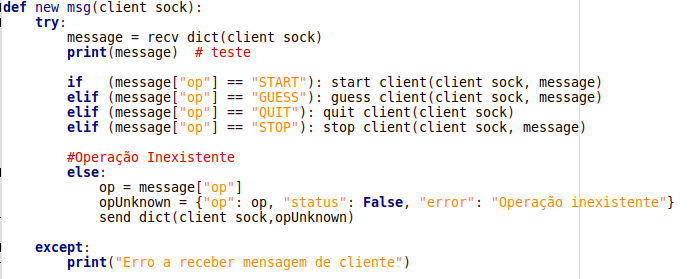
\includegraphics[width=10cm]{def-new-msg}
	\caption{Função new\_msg()\\}
	\label{fig:def-new-msg}
\end{figure} 

A função start\_client() é invocada sempre que o Cliente envia a operação Start.
Esta é a função que inicializa o jogo e começa por verificar se o Cliente que fez o pedido tem um ID válido (diferente de todos os jogadores activos). Se o Cliente tiver um ID válido são gerados aleatoriamente o número secreto e o número de tentativas e é iniciada a contagem de tentativas. Seguidamente adicionam-se os dados do Cliente ao dicionário Gamers. É através deste dicionário que a função start verifica se o Cliente tem ou não um ID válido e é também através dele que todas as outras funções verificam se as mensagens recebidas provêm de Clientes activos ou não.
Se o Cliente for válido o Servidor envia uma mensagem ao Cliente a informar que o jogo iniciou, juntamente com o número máximo de tentativas. Se isto não for verdade o Servidor envia uma mensagem de erro.

\begin{figure}[H]
	\centering
	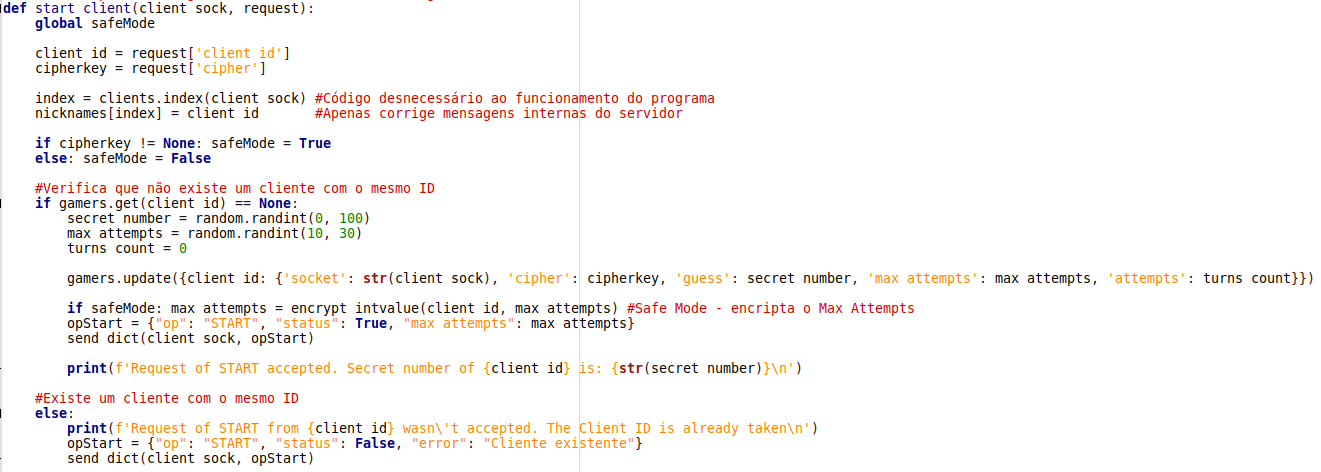
\includegraphics[width=10cm]{def-start}
	\caption{Função start\_client()\\}
	\label{fig:def-start}
\end{figure} 

A função guess\_client() é invocada sempre que o Cliente envia a operação Guess. Esta função deve ser utilizada sempre que o usuário faz uma tentativa de jogo.
Inicialmente, a função verifica se o Cliente que fez o pedido está registado como um jogador activo. Para fazer isso é invocada a função find\_client\_id.
Se o Cliente não estiver registado é lhe enviada uma mensagem de erro. Caso contrário, o programa regista a tentativa incrementando o número de jogadas feitas associadas ao Cliente (através do dicionário gamers).
Seguidamente, o Servidor compara o número adivinhado com o número secreto associado ao Cliente (através do dicionário gamers) e envia uma mensagem com o resultado dessa comparação(smaller/larger/equals)

\begin{figure}[H]
	\centering
	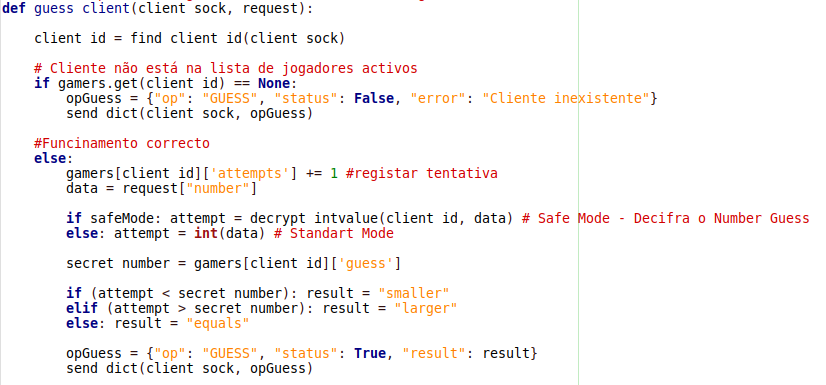
\includegraphics[width=10cm]{def-guess}
	\caption{Função guess\_client()\\}
	\label{fig:def-guess}
\end{figure} 

A função find\_client\_id() é chamada para obter um ID duma socket em específico. Esta função consiste em iterar todos os IDs registados no dicionário gamers e suas sockets verificando se existe uma socket igual à que fez o pedido. Se tal for o caso, a função retorna o ID pretendido, caso contrário envia None.

\begin{figure}[H]
	\centering
	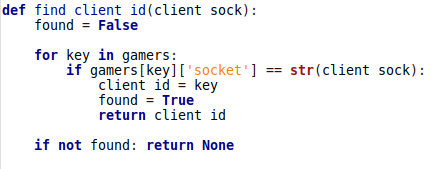
\includegraphics[width=10cm]{def-find}
	\caption{Função find\_client\_id()\\}
	\label{fig:def-find}
\end{figure} 

A função quit\_client() é invocada sempre que o Cliente envia a operação Quit. Esta função deve ser utilizada sempre que o usuário pretende desistir do jogo e apenas verifica se o Cliente que fez o pedido estava registado na lista de jogadores activos. 
Nesse caso, actualiza o ficheiro csv com o resultado "QUIT", envia uma mensagem indicando que a operação teve sucesso e elimina o jogador do dicionário gamers. Se este não estava registado o Servidor envia uma mensagem de erro

\begin{figure}[H]
	\centering
	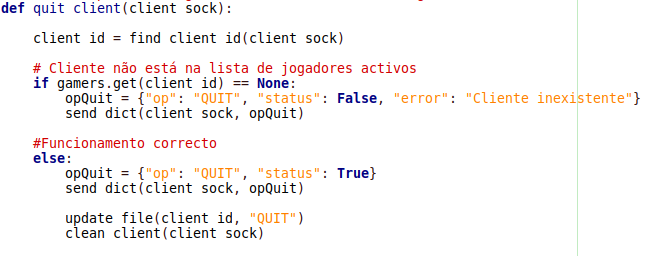
\includegraphics[width=10cm]{def-quit}
	\caption{Função quit\_client()\\}
	\label{fig:def-quit}
\end{figure} 

\clearpage

A função stop\_client() é invocada sempre que o Cliente envia a operação Stop. Esta função deve ser utilizada sempre que o usuário termina o jogo normalmente e começa por verificar se o Cliente que fez o pedido estava registado na lista de jogadores activos. Além disso, verifica se o número de tentativas registadas pelo Servidor é igual ao número de tentativas reportadas pelo Cliente.
Se não encontrar nenhum problema, verifica se o último número jogado é igual ao número secreto. Se tal for verdade significa que o jogador ganhou e actualiza o ficheiro csv com o resultado "SUCESS". Caso contrário, significa que o jogo terminou por esgotamento de tentativas e neste caso o ficheiro é actualizado com o resultado "FAILURE".


\subsubsection{Aplicação-Cliente}
A iniciação da aplicação-Cliente é feita com a invocação da função \textcolor{red}{main()} (última linha de código do programa) com recurso à variável \_\_main\_\_ , permitindo que o  código Python seja executado diretamente pelo Cliente como programa e não como módulo. Inicialmente, a função \textcolor{green}{main()} verifica os argumentos de entrada que o usuário inseriu para executar a sua conexão ao Servidor. Caso os argumentos inseridos estejam incorrectos o programa apresenta uma mensagem de erro e termina. 

\begin{itemize}
	\item\textsl{Cliente insere um número inválido de argumentos:} Para executar uma conexão comum  o usuário terá sempre que inserir 4 argumentos, tal como demonstrado anteriormente na figura \ref{fig:conexão-bem-executada1}. Caso um destes argumentos não seja especificado a função main detecta o erro recorrendo a um ciclo \textcolor{blue}{if}, comparando assim o número de argumentos inseridos (\textcolor{red}{len}(sys.argv)) com o número de argumentos esperados (4). Caso o número de argumentos inseridos seja diferente de 4 (!=4), o programa executa um \textcolor{blue}{print} da mensagem \textcolor{orange}{Erro1} e nega o acesso do Cliente ao Servidor através de \textcolor{blue}{sys.exit()}, tal como demonstrado na figura. \ref{fig:client_main_error_handling}.
	\item\textsl{Cliente insere argumento para porto não numérico ou numérico não inteiro:} Neste caso, o Cliente indicou um valor de entrada não numérico ou numérico inteiro real para especificar o porto de conexão ao Servidor. Assim, o Servidor executa o \textcolor{blue}{print} da mensagem \textcolor{orange}{Erro2} e nega o acesso do Cliente ao Servidor através de \textcolor{blue}{sys.exit()}, tal como demonstrado na figura \ref{fig:client_main_error_handling}.
\end{itemize}

\begin{figure}[H]
	\centering
	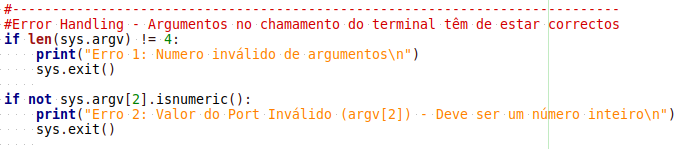
\includegraphics[width=10cm]{client_main_error_handling}
	\caption{Tratamento de erros de argumentos.\\}
	\label{fig:client_main_error_handling}
\end{figure} 

\clearpage

Se não houve nenhum erro na invocação do programa, o Cliente usa os argumentos de entrada dados pelo usuário para definir as suas variáveis \textbf{PORT} e \textbf{IP} e criar a socket (veriàvel \textsl{client\_ sock}) necessária à conexão usando a família \ac{afinet}, orientado à ligação \ac{str} em protocolo \ac{tcp}, tal como definido no Servidor: \textbf{client\_ sock = socket.socket(socket.AF\_ INET, socket.SOCK\_ STREAM)}. \\
Posteriormente, tenta executar uma conexão válida usando as variáveis \textbf{PORT} e \textbf{IP} definidas anteriormente, verificando as excepções destas variáveis, tal que:

\begin{itemize}
	\item\textsl{Exceção OverflowError:} Neste caso o usuário inseriu um porto cujo número é "out of range" do permitido, ie, o usuário deve inserir um número inteiro entre 1024 e 65535, pois o sistema tem apenas 65535 portos e os de valores inferiores a 1024 são portos já utilizados pelo sistema (\textbf{Well-Known Ports}). Assim, o sistema detecta a excepção e executa um \textcolor{blue}{print} da mensagem \textcolor{orange}{Erro2} onde indica que o valor do argumento 2 \textbf{PORT} é inválido, indicando os valores dentro do alcance permitido. 
	\item\textsl{Exceção gaierror:}  Neste caso, o usuário insere um valor \textbf{IP} inválido, sendo que o programa detecta o erro e executa um \textcolor{blue}{print} da mensagem \textcolor{orange}{Erro2} onde indica que o argumento 3 \text{IP} tem valor inválido.
	\item\textsl{ConnectionRefusedError:} Neste caso, o usuário inseriu todos os argumentos de entrada correctamente, contudo o valor d porto especificado não é o valor definido pelo Servidor, negando assim a conexão. Assim, o programa executa um \textcolor{blue}{print} da mensagem \textcolor{orange}{Erro2} onde indica que o porto especificado é incorrecto, pedindo ao utilizador que tente nova conexão com um porto válido (i.e. correcto).		 
\end{itemize}

\begin{figure}[H]
	\centering
	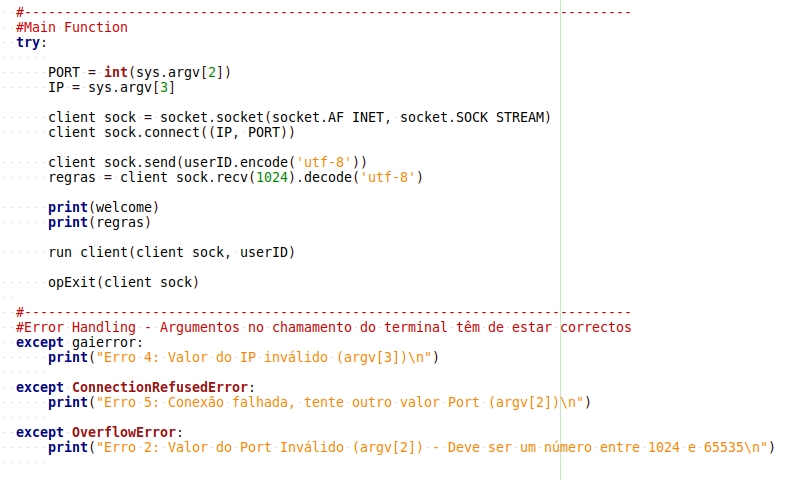
\includegraphics[width=10cm]{client_try_main}
	\caption{Tratamento da excepções da função main.\\}
	\label{fig:client_try_main}
	\flushleft\small\textit{}
\end{figure} 

\clearpage

Caso nenhum erro/exceção tenha sido detectado o cliente irá enviar o seu userID (variável global de argumento 1, ver figura \ref{fig:welcome}) para servidor usando metodo \textsl{encode} em \ac{utf8} e recorrendo à função \textbf{send}. Posteriormente recebe as regras do jogo em 1024 caracteres, das quais irá executar \textsl{decode} em \ac{utf-8}. É feito um \textcolor{blue}{print} de boas-vindas defenido na variàvel global "welcome" e das regras do jogo recebidas do servidor e definidas na variável "REGRAS" da função \textcolor{red}{main()} do servidor (figura \ref{fig:welcome}). Seguidamente é invocada a função run\_ client com os parametros socket (i.e. client\_ sock) e userID (figura \ref{fig:client_try_main2}.\\

\begin{figure}[H]
	\centering
	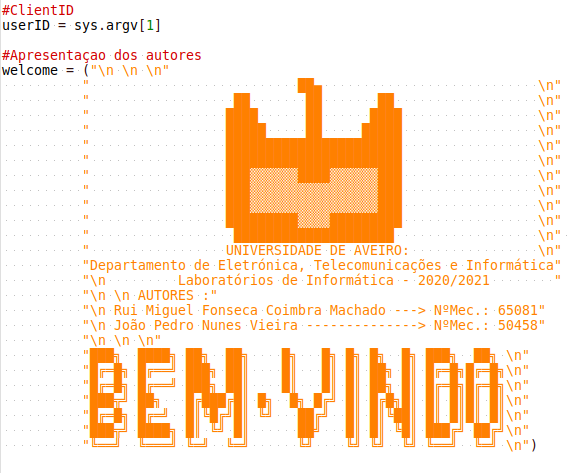
\includegraphics[width=10cm]{welcome}
	\caption{Mensagem de boas-vindas e variável global userID.\\}
	\label{fig:welcome}
	\flushleft\small\textit{A mensagem de boas-vindas contem a identificação dos autores deste trabalho por forma a ser identificado pelo utilizador com facilidade.}
\end{figure} 

\begin{figure}[H]
	\centering
	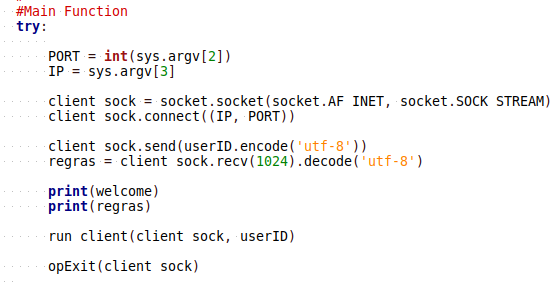
\includegraphics[width=10cm]{client_try_main2}
	\caption{Função main de cliente.\\}
	\label{fig:client_try_main2}
	\flushleft\small\textit{Nota: A operação \textbf{opExit(client\_sock)} não tem qualquer influencia no código. Apenas foi mantida por estar presente nos ficheiros fornecidos pelos docentes da \ac{uc}.}
\end{figure} 

\newpage
\subsubsection{Cliente: Funções de suporte}
Durante a execução da função \textbf{run\_clinet()} são usadas as seguintes funções (ilustradas nas figuras \ref{fig:client_exit_quit_retry}, \ref{fig:validate_response}): \\
\begin{itemize}
	\item\textsl{Função \textbf{opExit(client\_sock)}:} Quando invocada para o argumento de entrada client\_sock, a função executa um \textcolor{blue}{print} da mensagem de despedida (\textcolor{orange}{Até à próxima}), fecha o socket do cliente (client\_sock) e executa a operação de saida \textbf{sys.exit(0)}.
	\item\textsl{Função \textbf{validate\_response(client\_sock, response)}:} Verifica se a resposta do servidor é válida ou é uma mensagem de erro actua da seguinte forma. Se a resposta do servidor for válida (\textit{True}) então a função não faz nada de concreto, permitindo a sua passagem e display. Contudo se a resposta do servidor não for válida (ie. \textit{False}) a função faz o display da resposta bem como executa \textcolor{blue}{print} de mensagens de erro ("Operação não aceite" e "Operação inválida") invocando a função opExit para o client\_sock .
	\item\textsl{Função \textbf{opQuit(client\_sock)}:} É utilizada para, como o nome indica, executar a saida do cliente do programa. Quando invocada, gera um dicionário opQuit que envia como pedido ao servidor e recebe a resposta de aceitação de pedido. Seguidamente faz invocação da função \textsl{validate\_response} que valida a resposta do servidor e para  finalizar executa a invocação da função \textbf{opExit(client\_sock).}
	\item\textsl{Função \textbf{retry\_game(client\_sock, client\_id)}:} Esta função será usada pelo cliente para disponibilizar ao utilizador a opção de poder voltar a jogar novamente caso o jogo tenha terminado por vitória ou derrota (SUCCESS/FAILURE). Assim, quando invocada, faz uso de um ciclo \textcolor{blue}{while True} , no qual faz um \textcolor{blue}{Print} com uma pergunta ("Jogar Novamente?") e instruções para a resposta. Seguidamente, cria uma variável replay que requer um input por parte do utilizador, que ignora letras minusculas transformando-as em letras maiusculas para serem usadas como factor de selecção de resposta. Recorrendo a ciclo \textcolor{blue}{if}, a resposta é tratada de diferentes formas:
	\begin{itemize}
		\item\textbf{{Cliente responde "Y":}} Se o cliente responder "Y", será invocada novamente a função \textbf{run\_client} usando como paramentros de entrada client\_sock e client\_id, fazendo assim um novo jogo para o cliente.
		\item\textbf{{Cliente responde "N":}} Se o cliente responder "N", será executado um \textcolor{blue}{print} com uma mensagem de despedida e é invocada a função \textbf{opExit}.
		\item\textbf{{Cliente responde algo inválido:}} Se o cliente responder algo que não seja "Y" ou "N" , é ser executado um \textcolor{blue}{print} com uma mensagem de erro (\textcolor{orange}{Resposta Inválida}) e o cliente terá que executar novo input com uma resposta correcta (Y/N).
	\end{itemize}
\end{itemize}	


\begin{figure}[H]
	\centering
	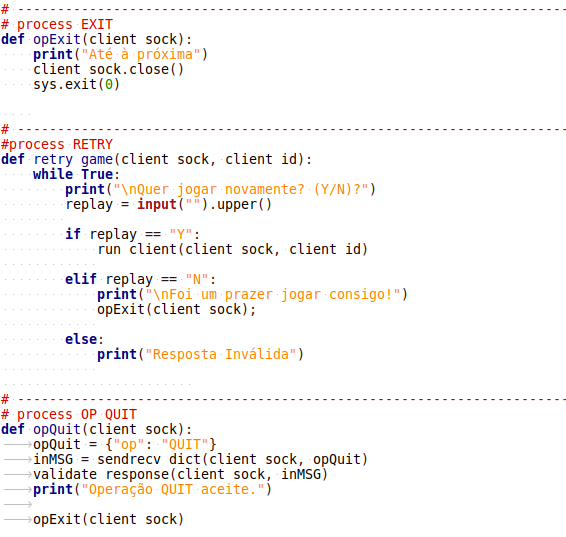
\includegraphics[width=8cm]{client_exit_quit_retry}
	\caption{Funções de suporte: opExit, opQuit e retry\_game .\\}
	\label{fig:client_exit_quit_retry}
\end{figure} 
\begin{figure}[H]
	\centering
	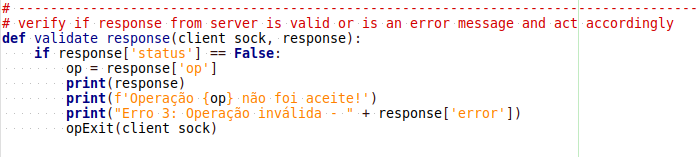
\includegraphics[width=8cm]{validate_response}
	\caption{Função de suporte: validate\_response .\\}
	\label{fig:validate_response}
\end{figure} 

Finalmente, é descrita a implementação das funções \textbf{initQuestion} e \textbf{opGuessing}, cujas ilustrações se encontram nas figuras \ref{fig:initQuestion}, \ref{fig:opGuessing}.
\begin{itemize}
	\item\textsl{Função \textbf{initQuestion()}:} É usada para perguntar ao usuário o modo de inicialização que deseja utilizar. Assim, recorrendo a um ciclo \textcolor{blue}{while True} a função recorre a um \textcolor{blue}{print} fazendo display de uma questão de escolha de modo de iniciação, sendo que seguidamente define uma variável \textbf{response} que requer um input por parte do utilizador (que ignora letras minusculas transformando-as em letras maiusculas) para serem usadas como factor de selecção de resposta. Recorrendo a ciclo \textcolor{blue}{if}, a resposta é tratada de diferentes formas:
	\begin{itemize}
		\item\textbf{{Cliente responde "Y":}} Se o cliente responder "Y", a função irá fazer um display de mensagem a confirmar a inicialização de modo de segurança e define a variàvel global safeMode com valor boolean \textbf{True}.
		\item\textbf{{Cliente responde "N":}} Se o cliente responder "N", a função irá fazer um display de mensagem a confirmar a inicialização de modo de standard (não seguro) e define a variàvel global safeMode com valor boolean \textbf{False}.
		\item\textbf{{Cliente responde algo inválido:}} Se o cliente responder algo que não seja "Y" ou "N" , é ser executado um \textcolor{blue}{print} com uma mensagem de erro (\textcolor{orange}{Resposta Inválida}) e o cliente terá que executar novo input com uma resposta correcta (Y/N).
	\end{itemize}			
		
	\item\textsl{Função \textbf{opGuessing(client\_sock, clientInput)}:} Esta função processa a opGuess. Inicialmente define as variáveis globais \textsl{turnCount}, \textsl{max\_attempts} e \textsl{safeMode}, definindo posteriormente a variável \textit{sucess} com valor boolean \textbf{False}, a qual vai ser usada como forma de verificar se a escolha do número do utilizador foi a correcta (igual a número secreto) ou não.\\
	Assim, recorrendo a ciclos \textcolor{blue}{if} a função irá triar a informação da seguinte forma:	
	\begin{itemize}
		\item\textbf{{Cliente escolhe um número inferior a 0 ou superior a 100:}} Neste caso a função faz o display de mensagem: \textcolor{orange}{A operação 'Guess' só aceita valores entre 0 e 100. Tente outra vez.}. Assim, o cliente é forçado a escolher novamente um numero que esteja dentro dos limites permitidos/desejados pelo jogo.
		\item\textbf{{Cliente escolhe um número adequado:}} A função gera um dicionário opGuess que envia como pedido ao servidor e recebe a resposta de aceitação de pedido e faz invocação da função \textsl{validate\_response} que valida a resposta do servidor. Posteriormente faz uma adiciona mais uma unidade à contagem de tentativas (\textsl{turnCount} e faz retira o resultado da mensagem do servidor (variável "inMSG") e executa o display do resultado obtido (\textsl{result)}), da contagem de tentativas (\textsl{turncount}) e do máximo de tentativas que o utilizador tem (\textsl{max\_attempts}).
		\begin{itemize}		
			\item\textbf{{Tratamento de dados (modo de segurança:}} Os dados serão colocados numa variável \textbf{data} e cifrados pela função \textbf{encrypt\_intvalue} usando como paramentros uma chave de cifra (\textsl{cipherkey}) gerada automáticamente e os seu número escolhido (\textsl{clientInput}). A função \textbf{encrypt\_intvalue} será discutida mais à frente na secção  \ref{sub.seg_implementação}.
			\item\textbf{{Tratamento de dados (modo standard:}} Os dados serão simplesmente aceites e enviados tal como estão, sendo colocados numa variável \textbf{data}.
		\end{itemize}		
		\item\textbf{{Cliente acertou no número secreto:}} Se o cliente acertar no número secreto (result == "equals"), a função altera o valor booleano da sua variável "sucess" para \textbf{True}.	

	\end{itemize}		
\end{itemize}

\begin{figure}[H]
	\centering
	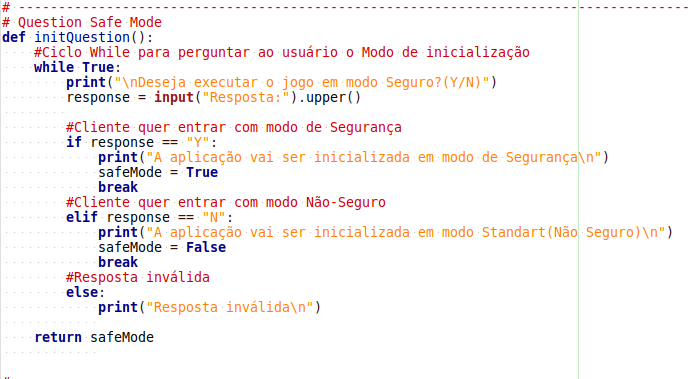
\includegraphics[width=8cm]{initQuestion}
	\caption{Função de suporte: initQuestion .\\}
	\label{fig:initQuestion}
\end{figure} 
\begin{figure}[H]
	\centering
	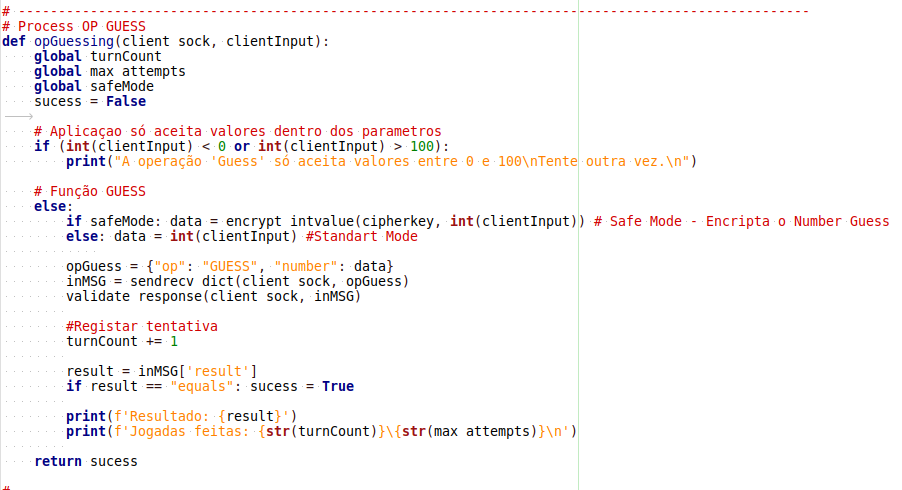
\includegraphics[width=8cm]{opGuessing}
	\caption{Função de suporte: opGuessing .\\}
	\label{fig:opGuessing}
\end{figure} 

\subsubsection{Cliente: Função run\_client}
A função \textbf{run\_client} tem como argumentos de entrada o client\_sock e o client\_id. Após ser invocada pela função \textcolor{red}{main()}, a função define variáveis globais \textsl{turnCount}, \textsl{max\_attempts}, \textsl{safeMode}, \textsl{cipherkey} definindo posteriormente as variáveis \textit{skip}, \textit{sucess} (ambas com valores boolean \textbf{False}) e \textit{turnCount = 0}. \\
Posteriormente usa a variável \textsl{safeMode} para invocar a função \textbf{initQuestion()}, por forma a dar ao utilizador a opção de escolher entre \textit{modo standard} ou \textit{modo de segurança}. Se for escolhido \textit{modo de segurança} (safeMode == True) será gerada uma \textsl{cipherkey} aleatória de 16 bits a qual será posteriormente usada para cifrar os dados comunicados entre Cliente e Servidor, sendo criada uma variável \textsl{cipherkey\_send} que será codificada em base64 (para ser compativel com \ac{json}).
	Seguidamente o Cliente irá executar a função \textbf{opStart} da seguinte forma:

	\begin{itemize}		
			\item\textbf{Modo de Segurança:} A operação \textbf{opStart} será executada enviando ao Servidor, para além do client\_id , a \textit{cipherkey\_tosend} gerada anteriormente. 
			\item\textbf{Modo Standard:} A operação \textbf{opStart} será executada enviando ao Servidor apenas o client\_id tendo o valor da cifra \textit{None}.
	\end{itemize}
	
	\textsl{Nota: Em todas as etapas da função \textbf{run\_client}, caso o utilizador tenha optado pelo \textit{modo de segurança}, os dados comunicados entre as aplicações Cliente-Servidor serão cifrados no envio e decifrados na recepção, por forma a obter uma conexão segura.}

\begin{figure}[H]
	\centering
	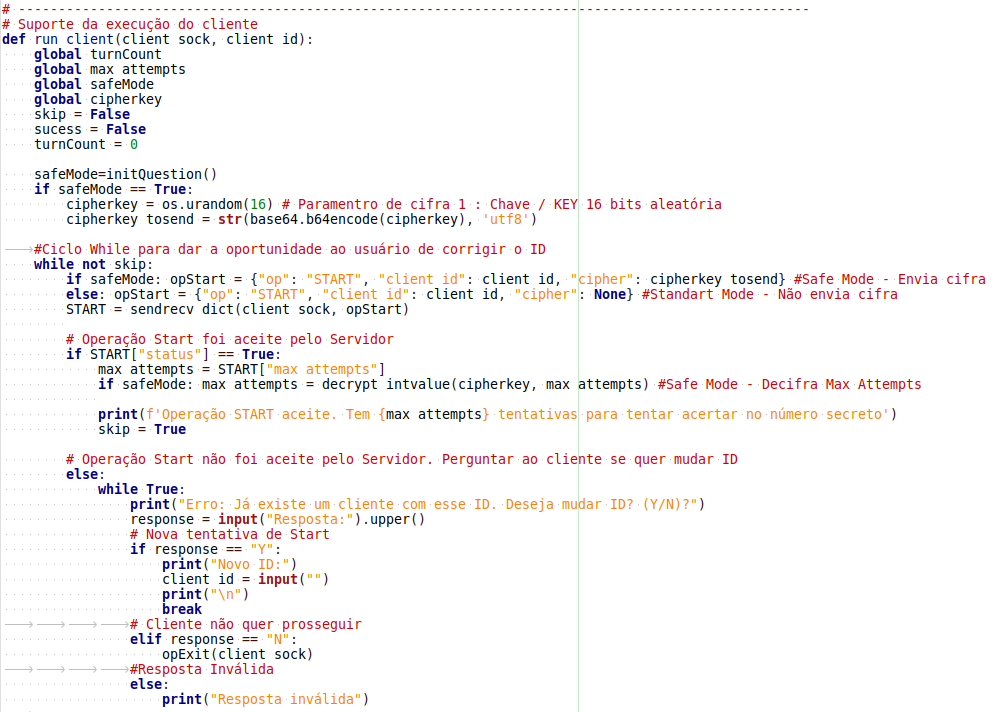
\includegraphics[width=8cm]{run_client1}
	\caption{Função run\_client - Parte 1 .\\}
	\label{fig:run_client1}
\end{figure} 

\begin{figure}[H]
	\centering
	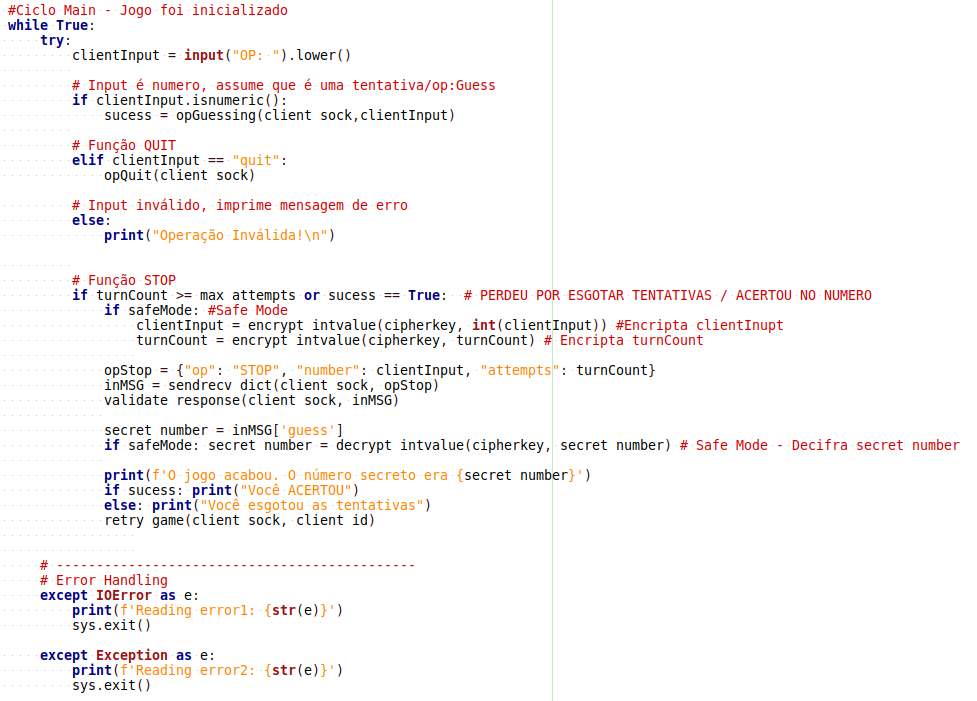
\includegraphics[width=8cm]{run_client2}
	\caption{Função run\_client - Parte 2 .\\}
	\label{fig:run_client2}
\end{figure} 

%%%%%
\section{Segurança}
\label{sec.segurança}
A transmissão entre Cliente (pedidos) e Servidor (respostas), são cifrados por cifras simétricas por blocos \ac{aes-128} em modo \ac{ecb}.´

\subsection*{Implementação}
\label{sub.seg_implementação}
Nesta secção iremos abordar as funções de segurança implementadas nas aplicações Cliente-Servidor:

\subsubsection{Server:}
No servidor, existem três funções implementadas para a segurança: \textbf{encrypt\_intvalue}, \textbf{decrypt\_intvalue} e \textbf{find\_cipher}. A implementação destas funções será abeguidamente e pode ser visualizada na figura \ref{fig:server_segurança}:
	\begin{itemize}
		\item\textbf{Função \textbf{find\_cipher}:} Serve para encontrar a (\textit{cipherkey}) do cliente com determinado userID, ie., a função faz uma busca no dicionário gamers pela referencia \textit{cipher} para obter a cipherkey correspondente ao \textit{client\_id} do cliente em questão. Posteriormente faz o decode() de base64 e obtem a cipherkey pronta a ser usada para criar a cifra (\textit{cipher} = AES.new(cipherkey, mode)) em modo \ac{ecb} (mode = AES.MODE\_ECB) e propagar esta através do \textcolor{blue}{return}.
		
		\item\textbf{Função \textbf{encrypt\_intvalue(client\_id, data)}:} De argumentos de entrada \textit{client\_id} e \textit{data}, esta função obtem a cifra do cliente invocando a função \textbf{find\_cipher} com o client\_id pretendido. Seguidamente, os dados (varável \textit{data}) são cifrados numa string binária de 128 bits (16 octetos) em \ac{utf-8}, sendo posteriormente usados para criar uma nova variável \textit{data\_tosend} codificando a mesma em base64 modo \ac{utf-8}. Finalmente os dados a enviar (\textit{data\_tosend}) são retornados  através de \textcolor{blue}{return}.
		\item\textbf{Função \textbf{decrypt\_intvalue}:} Similar à função anteior, a função \textbf{decrypt\_intvalue} tem argumentos de entrada \textit{client\_id} e \textit{data} e obtem a cifra do cliente invocando a função \textbf{find\_cipher} com o client\_id pretendido. Posteriormente executa o decode de base64 dos dados (variável \textit{data}) e usa a cifra (\textit{cipher}) para decifrar os dados. Finalmente cria uma nova variável para dados a enviar chamada \textit{data\_tosend} a qual converte os dados novamente para integer e propaga os dados fazendo uso do \textcolor{blue}{return}.		
	\end{itemize} 
	
\begin{figure}[H]
	\centering
	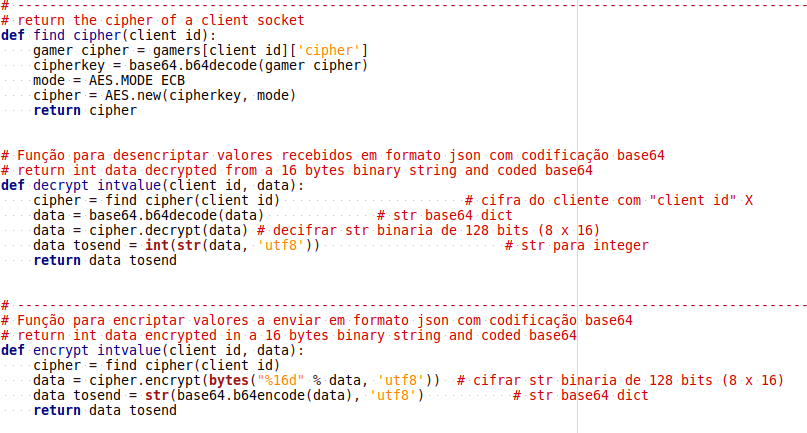
\includegraphics[width=8cm]{server_segurança}
	\caption{Funções de segurança: Servidor.\\}
	\label{fig:server_segurança}
\end{figure} 

\subsubsection{Cliente:}
No Cliente, existem duas funções implementadas para a segurança: \textbf{encrypt\_intvalue}, \textbf{decrypt\_intvalue}, sendo a geração de uma cipherkey feita dentro da função \textbf{run\_client} tal como descrito na secção \ref{sub.run_client}. A implementação destas funções será abeguidamente e pode ser visualizada na figura \ref{fig:cliente_segurança}:
	\begin{itemize}
		\item\textbf{Função \textbf{encrypt\_intvalue}:} de argumentos de entrada \textit{client\_id} e \textit{data}, a função cria uma variável que define o modo \ac{ecb} a utilizar (mode = AES.MODE\_ECB) que usa juntamente com a cipherkey criada no decorrer da função run\_client , para gerar uma cifra na varável \textit{cipher} que usa para cifrar os  dados contidos na variável \textit{data} numa string de 128 bits (16 octetos). Posteriormente, cria uma variável \textit{data\_tosend} a qual faz e guarda uma cópia dos dados presentes na variàvel \textit{data} fazendo o encode de base64 e é propagada no \textcolor{blue}{return}.		
		\item\textbf{Função \textbf{decrypt\_intvalue}:}de argumentos de entrada \textit{client\_id} e \textit{data}, a função cria uma variável que define o modo \ac{ecb} a utilizar (mode = AES.MODE\_ECB) que usa juntamente com a cipherkey, criada no decorrer da função run\_client, para gerar uma cifra na varável \textit{cipher}. Posteriormente  executa o decode de base64 dos dados da variável \textit{data} e usa a cifra criada para decifrar o seu conteudo. Posteriormente cria uma variável para dados a enviar chamada \textit{data\_tosend} a qual converte os dados novamente para integer e propaga os dados fazendo uso do \textcolor{blue}{return}.		
	\end{itemize} 

\begin{figure}[H]
	\centering
	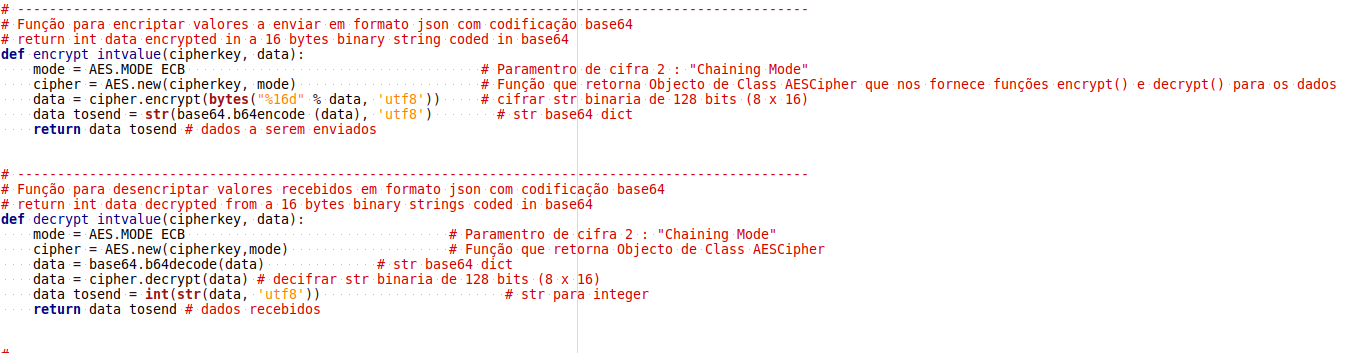
\includegraphics[width=8cm]{cliente_segurança}
	\caption{Funções de segurança: Cliente.\\}
	\label{fig:cliente_segurança}
\end{figure} 


%
%%%%%%%%%%%%%%%%%%%%%%%%%%%%%%%%%%%%%%%%%%%%%%%%%%%%%%%%%
%%%%%CAPÍTULO 2: TESTES E RESULTADOS
%
\chapter{Testes de Funcionalidade e Resultados}
\label{chap.testes e resultados}
\lhead{Testes de Funcionalidade e Resultados}

Além das normas de implementação da aplicação, o enunciado proposto continha regras para lidar com determinadas situações de erro e garantir que o programa funciona correctamente. Nesta secção serão abordados os testes realizados para confirmar que o código desenvolvido está preparado para lidar não só com essas situações mas também com outros erros que foram encontrados ao longo do processo.

\section{Invocação das aplicações}
\label{sec.testes-servidor}
Para inicializar o Servidor invoca-se o seguinte comando no terminal, como indicado na figura \ref{fig:abrir-servidor}: {\large\textsl{python3 server.py port}}. 

\begin{center}	
	\begin{figure}[H]
		\centering
		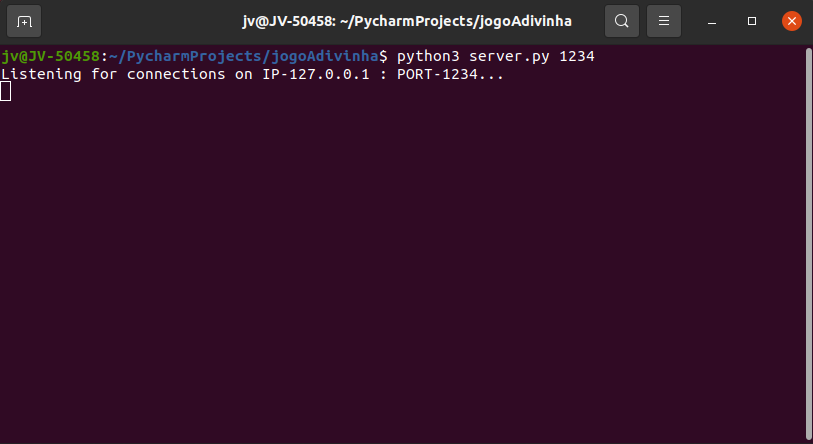
\includegraphics[width=10cm]{abrir-servidor}
		\caption{Exemplo iniciação de Servidor\\}
		\label{fig:abrir-servidor}
		\flushleft\small\textit{Nota: O Servidor encontra-se iniciado e à "escuta" de novos pedidos de conexão.}
	\end{figure}
\end{center}

Se o Servidor for inicializado com um número incorrecto de argumentos é apresentada uma mensagem de erro. Além disso, o argumento referente ao porto deve ser um número inteiro compreendido entre 1024 e 65535. Este limite deve-se ao facto de o sistema ter apenas 65535 portos e os de valores inferiores a 1024 já estão obrigatoriamente a ser utilizados pelo sistema (também conhecidas como \textit{Well-Known Ports}).

\begin{center}	
	\begin{figure}[H]
		\centering
		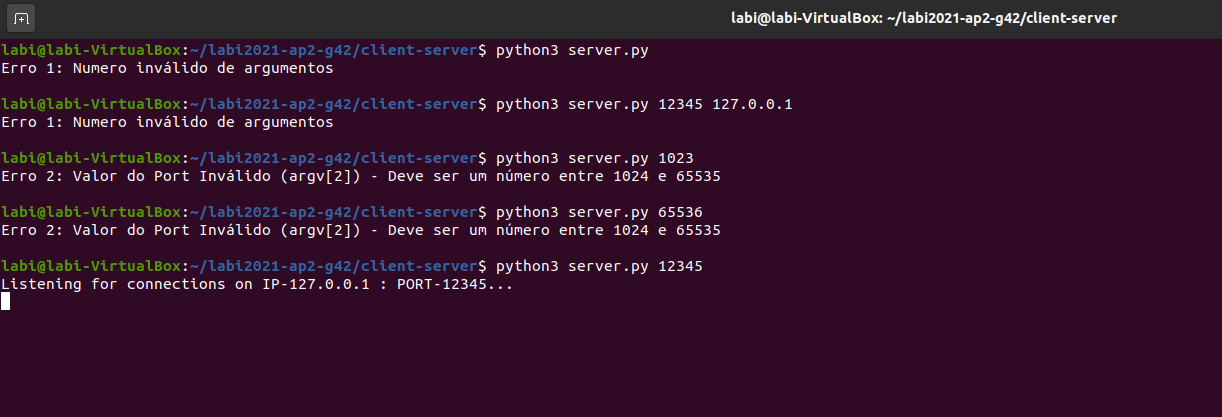
\includegraphics[width=10cm]{erro_sv_comando}
		\caption{Erros de comando\\}
		\label{fig:erro_sv_comando}
		\flushleft\small\textit{Nota: Poderiam ser usados portos entre 0 e 1023, contudo tal é desaconselhado uma vez que seria necessário "root privilege" do sistema operativo.}
	\end{figure}
\end{center}

A aplicação-Cliente também deve ser inicializada com um número correcto de argumentos, caso contrário é apresentada uma mensagem de erro. Quando é invocado o comando de inicialização do Cliente os argumentos referentes ao porto e ao IP também devem cumprir certos requisitos. No caso do porto, este já deve estar estabelecido para receber conexões e o argumento deve ser um número inteiro compreendido entre 1024 e 65535. No caso do IP, este deve ser invocado no formato X.X.X.X onde X representa um número inteiro entre 0 e 255.

\begin{center}
	\begin{figure}[H]
		\centering
		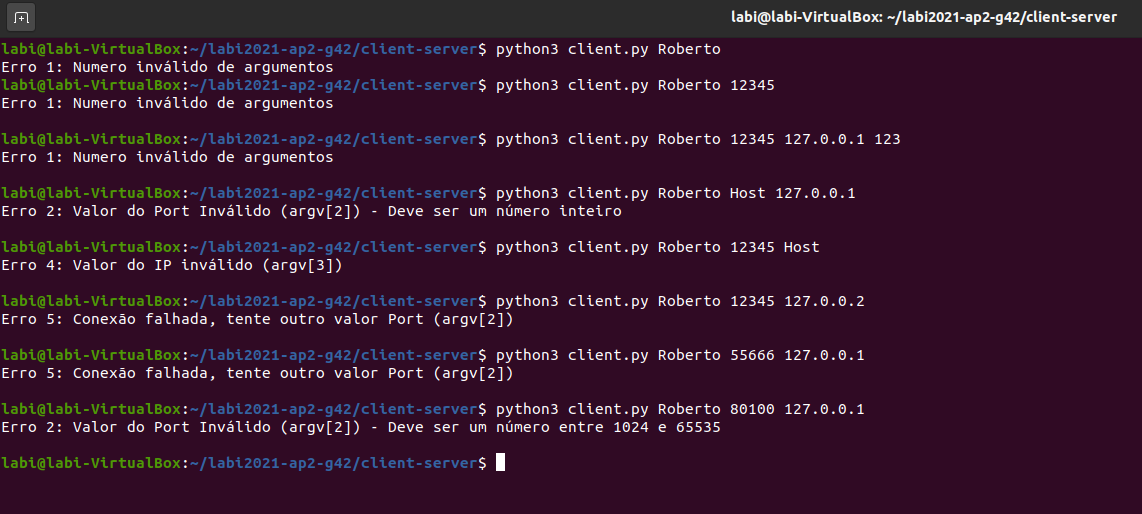
\includegraphics[width=10cm]{erro_cl_comando}
		\caption{Erros de comando\\}
		\label{fig:erro_cl_comando}
		\flushleft\small\textit{Nota: Tal como referido anteriormente, poderiam ser usados portos entre 0 e 1023, contudo tal é desaconselhado uma vez que seria necessário "root privilege" do sistema operativo.}
	\end{figure}
\end{center}
		


O Servidor deve ser desligado pela acção \textit{keyboard interrupt}, usando a combinação de teclas \textbf{ctrl + c}, ou simplesmente desligando a consola/terminal de comandos, como se pode constatar na figura \ref{fig:fechar-servidor}: 

\begin{center}	
	\begin{figure}[H]
		\centering
		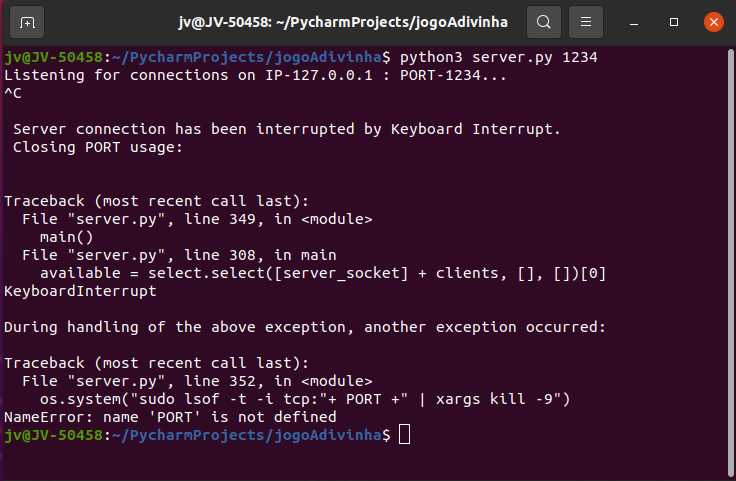
\includegraphics[width=10cm]{fechar-servidor}
		\caption{Fechar o servidor correctamente\\}
		\label{fig:fechar-servidor}
		\flushleft\small\textit{Nota: Como se pode verificar, o Servidor indica mensagem de "S\textit{erver connection has been interrupted}" fazendo de seguida o comando "\textit{kill -9}" para disponibilizar o porto utilizada.}
	\end{figure}
\end{center}

Caso sejam usados outro métodos, como a combinação de teclas \textbf{ctrl + z}, o uso do porto não é libertado para uso futuro, como demonstrado na figura \ref{fig:fechar-servidor-mal}:

\begin{center}	
	\begin{figure}[H]
		\centering
		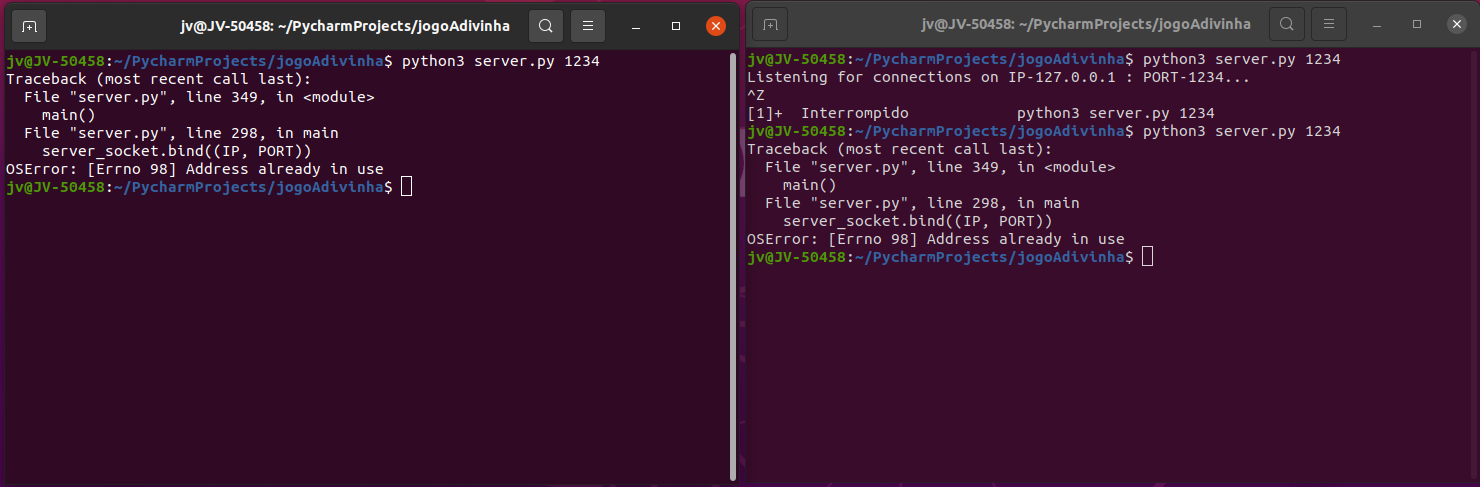
\includegraphics[width=10cm]{fechar-servidor-mal}
		\caption{Fechar o servidor de forma errada\\}
		\label{fig:fechar-servidor-mal}
		\flushleft\small\textit{Nota: Como se pode verificar, a consola/terminal da direita executou \textbf{ctrl + z} para fechar o Servidor, tendo como resultado nem este terminal ou outro poderem fazer uso do porto 1234}
	\end{figure}
\end{center}

Caso tal ocorra, existem duas alternativas simples de libertar o porto para uso futuro. A mais simples seria desligar o terminal inicialmente usado para correr o Servidor. Se isso não for o pretendido pode-se correr o comando demonstrado na figura \ref{fig:servidor-mal-fechado-kill}
\begin{center}	
	\begin{figure}[H]
		\centering
		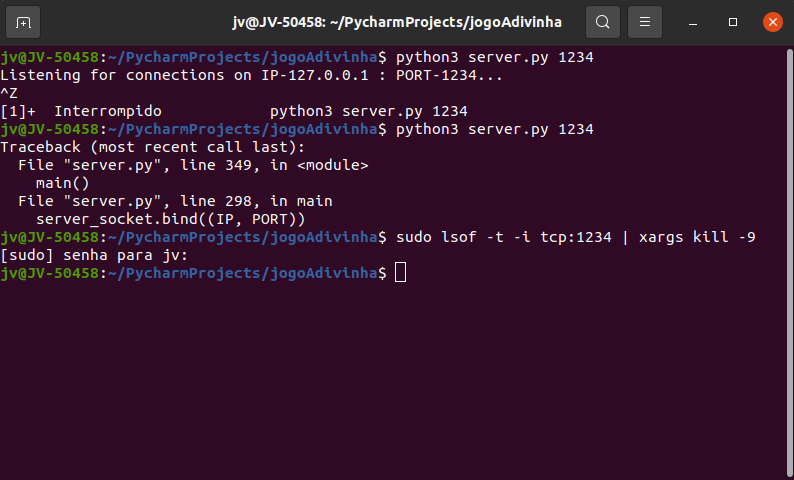
\includegraphics[width=10cm]{servidor-mal-fechado-kill}
		\caption{Disponibilizar porta via comando terminal linux.\\}
		\label{fig:servidor-mal-fechado-kill}
		\center\small\textit{Comando: sudo lsof -t -i tcp:port | xargs kill -9}
	\end{figure}
\end{center}

\section{Funcionalidade do Cliente}

O Servidor deve conseguir estabelecer conexão com vários Clientes ao mesmo tempo e garantir o correcto funcionamento do jogo para todos os usuários conectados, garantindo que nenhum usuário tenha de esperar que outros acabem para poder executar o jogo, como  demonstrado na figura \ref{fig:servidor-varios-clientes}

\begin{figure}[H]
	\centering
	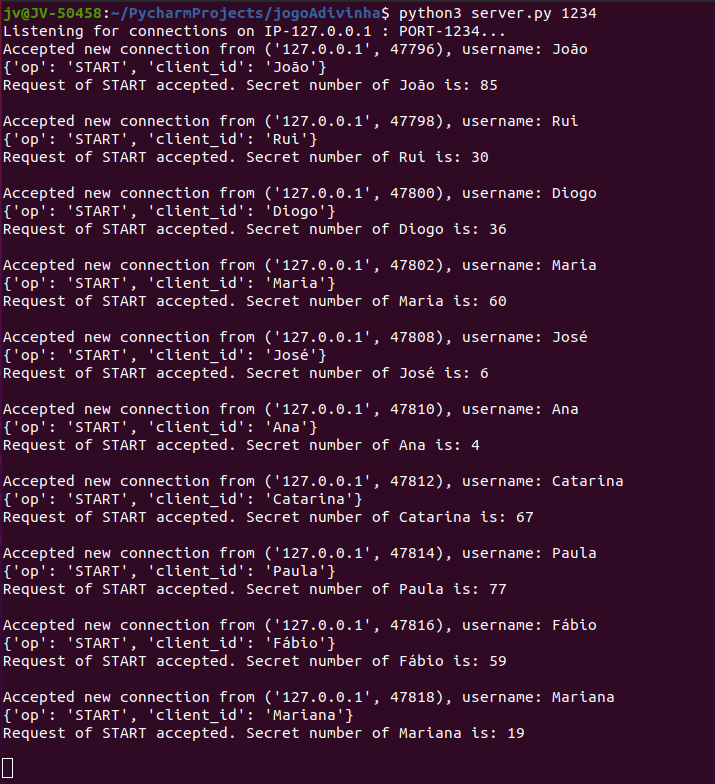
\includegraphics[width=8cm]{servidor-varios-clientes}
	\caption{Servidor com 10 clientes conectados ao mesmo tempo, com ID diferente uns dos outros\\}
	\label{fig:servidor-varios-clientes}
\end{figure}

O enunciado do trabalho não especifica o que a aplicação Servidor deve apresentar no seu terminal. Assim, decidiu-se que seria interessante o Servidor apresentar certas mensagens de forma a monitorizar algumas das suas operações internas.  

\begin{figure}[H]
	\centering
	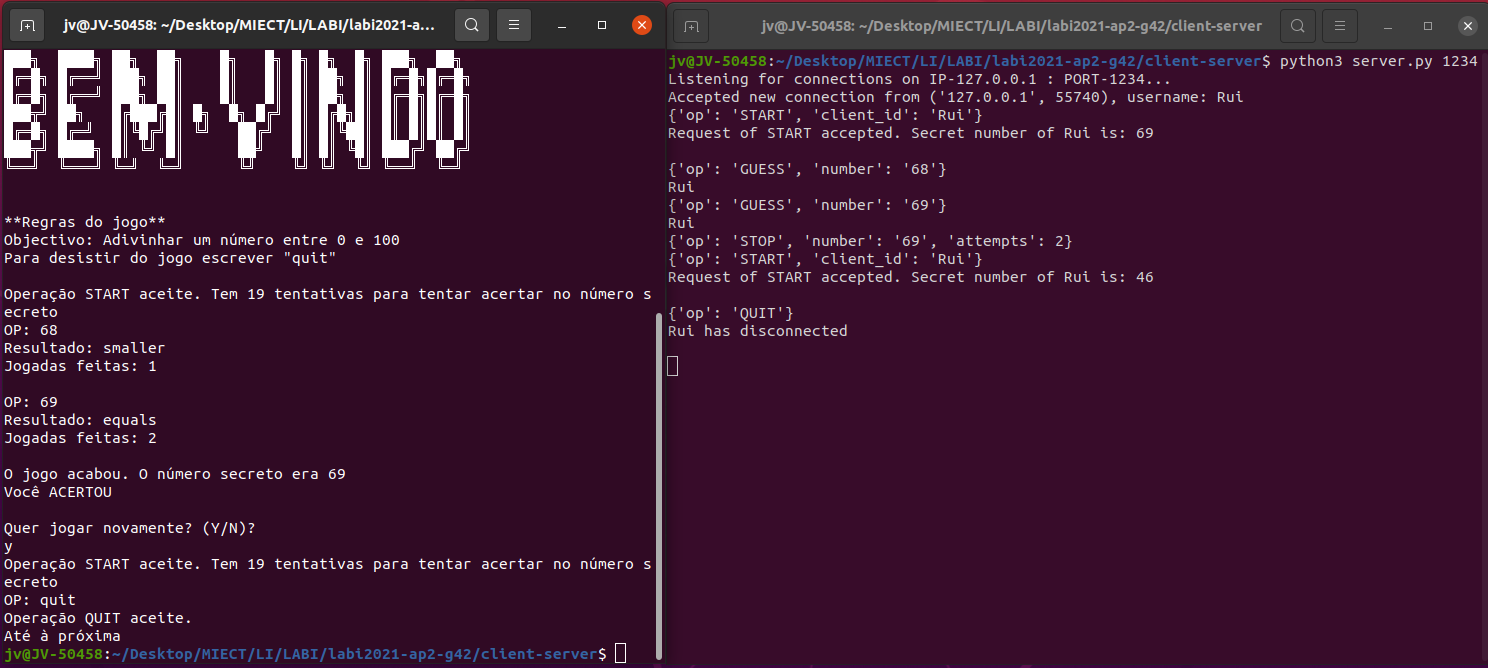
\includegraphics[width=10cm]{actividade-recente}
	\caption{Servidor: Actividade recente dos jogadores\\}
	\label{fig:actividade-recente}
\end{figure}

Após ser inicializado, o Cliente apresenta uma mensagem com as regras do jogo e envia automaticamente um pedido ao Servidor para começar o jogo. Se não existir nenhum usuário com o mesmo ID a jogar o Servidor aceita o pedido, caso contrário o Servidor envia uma mensagem a negar o pedido. Nesse caso, a aplicação-Ciente informa o usuário e pergunta-lhe se quer mudar o seu ID. O usuário pode trocar de ID até encontrar um válido ou sair da aplicação.

\begin{figure}[H]
	\centering
	\begin{subfigure}[t]{0.45\textwidth}
		\centering
		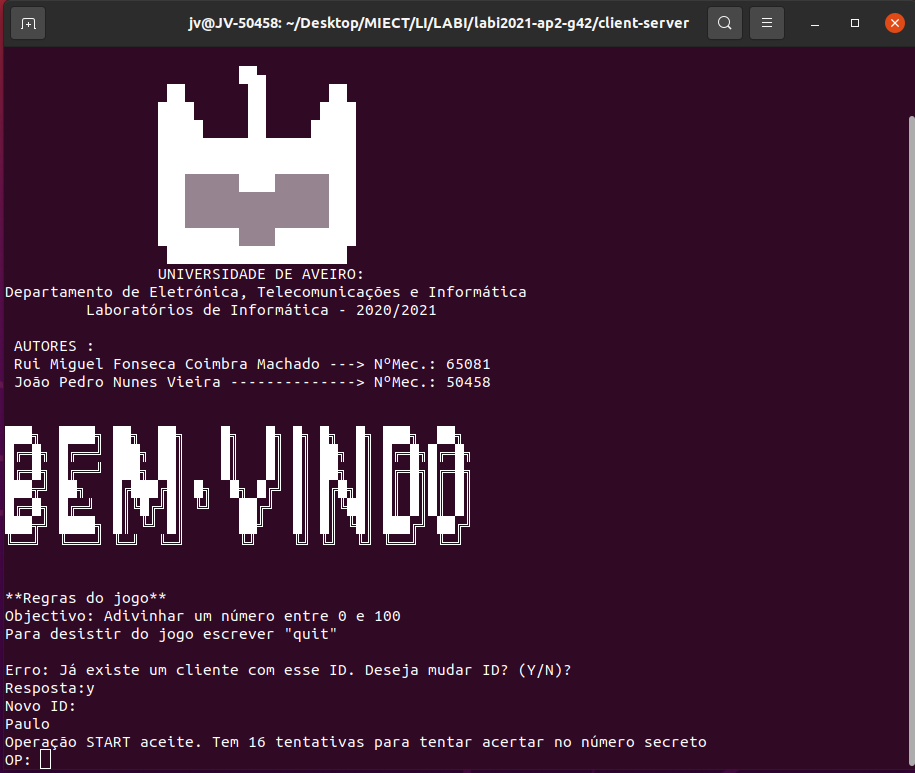
\includegraphics[scale=0.2]{cliente-muda-id}
		\caption{Cliente muda de ID}
		\label{fig:cliente-muda-id}
	\end{subfigure}
	\begin{subfigure}[t]{0.45\textwidth}
		\centering
		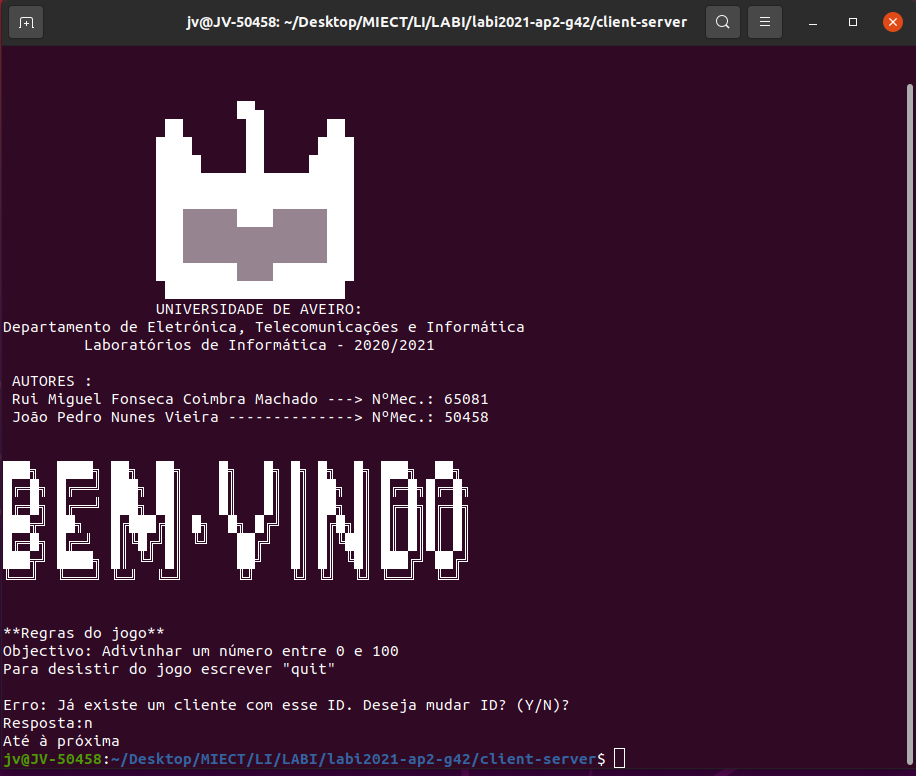
\includegraphics[scale=0.2]{cliente-não-muda-id}
		\caption{Cliente não muda de ID}
		\label{fig:cliente-não-muda-id}
	\end{subfigure}	
	\caption{ Cliente muda ou não muda de id  }
	\label{fig:mudar-id}
\end{figure}	

A escolha de um novo ID apenas ligeiramente diferente do ID já registado é permitido pelo Servidor, como exemplificado na figura \ref{fig:cliente-muda-id-sem-acento}:  

\begin{figure}[H]
	\centering
	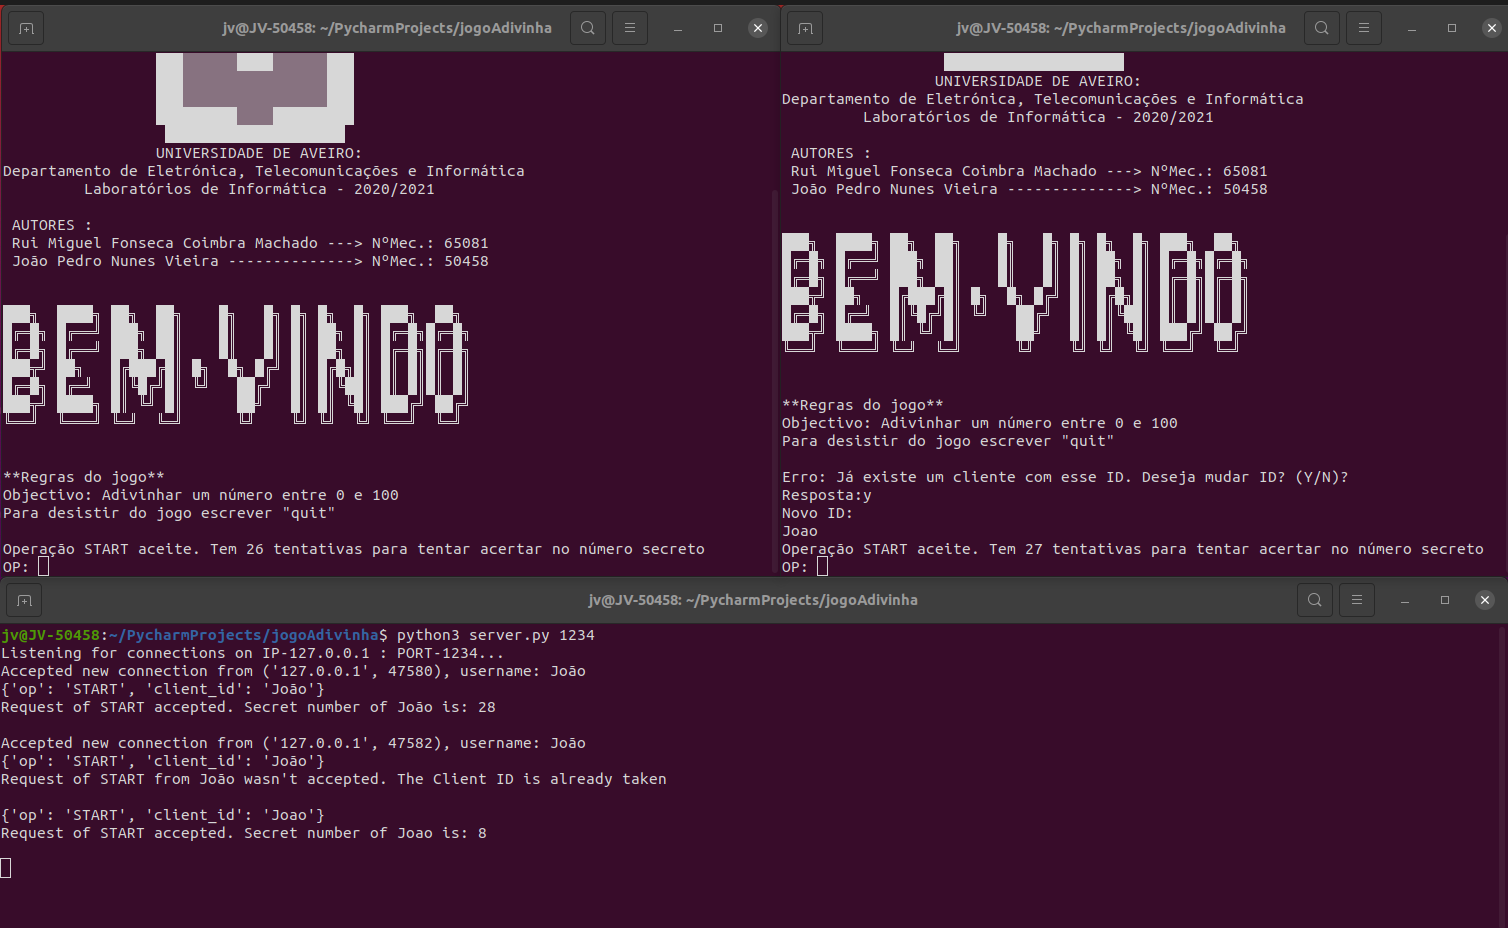
\includegraphics[width=12cm]{cliente-muda-id-sem-acento}
	\caption{Escolha de um novo ID similar a outro ID já registado\\}
	\label{fig:cliente-muda-id-sem-acento}
	\flushleft\small\textit{Nota: Desta forma, clientes podem escolher ID do estilo \textit{nickname} com caracteres diferentes}
\end{figure} 

Como já referido anteriormente, após o começo do jogo o usuário pode fazer várias tentativas para adivinhar o número secreto escrevendo um número compreendido entre 0 e 100 no terminal da aplicação-Cliente. O Servidor recebe a tentativa e retorna uma mensagem com informação relativa à mesma, dizendo se a tentativa está abaixo ou acima do número secreto, ou se acertou. Além disso, sempre que é feita uma tentativa a aplicação-Cliente apresenta no terminal o número de tentativas realizadas e o número máximo de tentativas possíveis.

\begin{figure}[H]
	\centering
	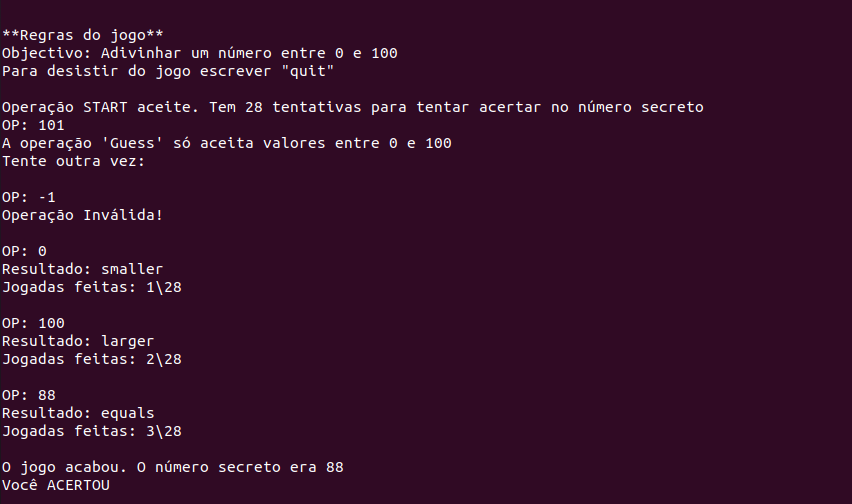
\includegraphics[width=12cm]{func_guess}
	\caption{Funcionamento da operação Guess\\}
	\label{fig:func_guess}
\end{figure} 

Se o usuário acertar no número secreto ou esgotar as suas tentativas a aplicação-Cliente apresenta uma mensagem com o resultado do jogo e o número secreto gerado pelo Servidor, perguntando ainda ao usuário se pretende jogar mais uma vez. O usuário pode começar um jogo novo ou terminar a aplicação.

\begin{figure}[H]
	\centering
	\begin{subfigure}[t]{0.45\textwidth}
		\centering
		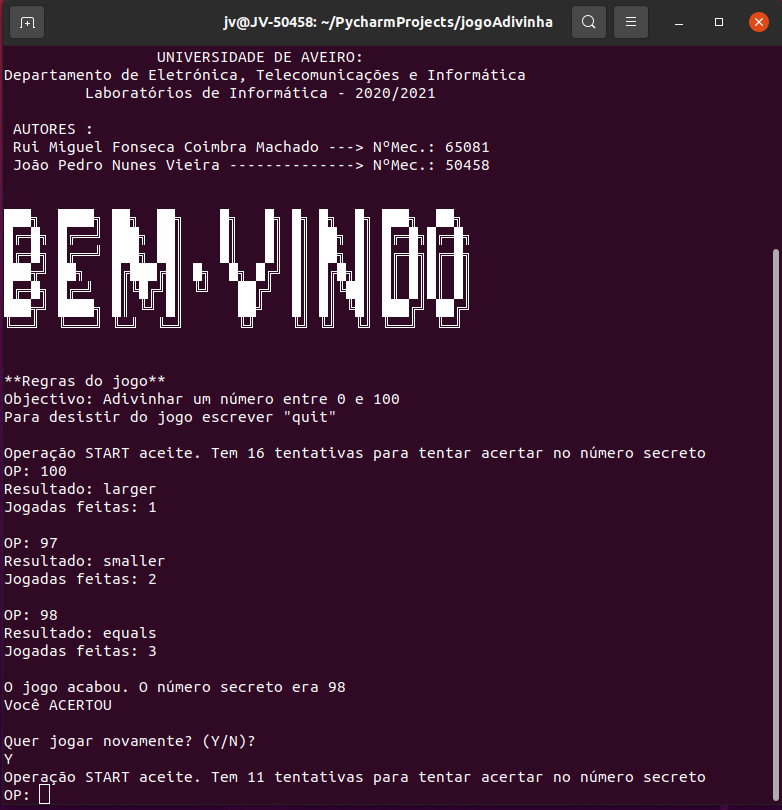
\includegraphics[scale=0.2]{jogo-ganha-y}
		\caption{Jogo completo. Cliente ganhou e escolhe jogar novamente}
		\label{fig:jogo-ganha-y}
	\end{subfigure}
	\begin{subfigure}[t]{0.45\textwidth}
		\centering
		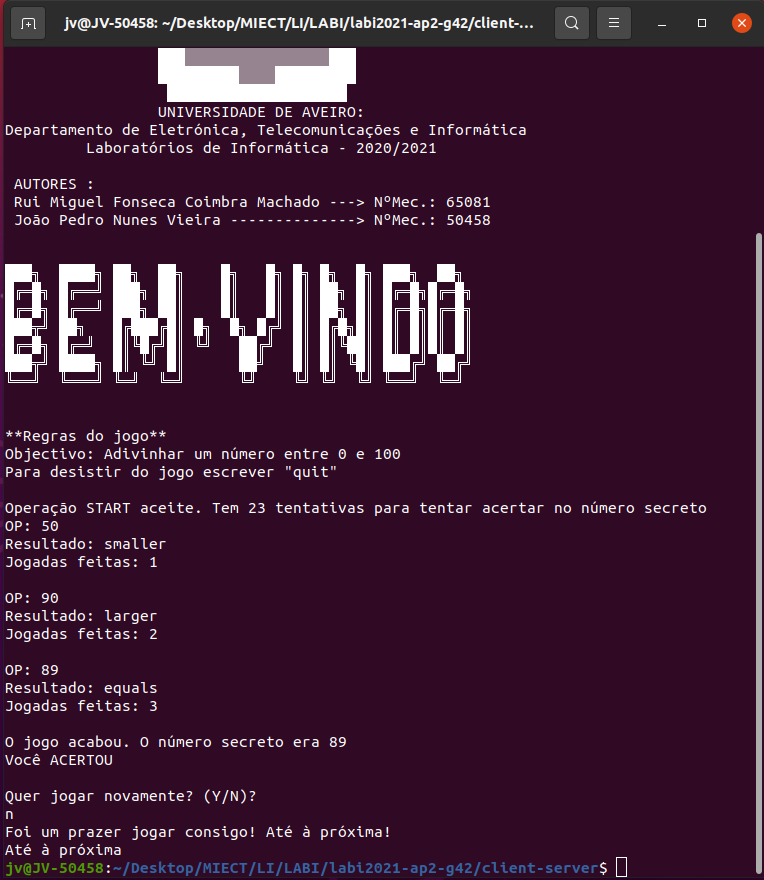
\includegraphics[scale=0.2]{jogo-ganha-n}
		\caption{Jogo completo. Cliente ganhou e escolhe não jogar novamente}
		\label{fig:jogo-ganha-n}
	\end{subfigure}	
	\begin{subfigure}[t]{0.45\textwidth}
		\centering
		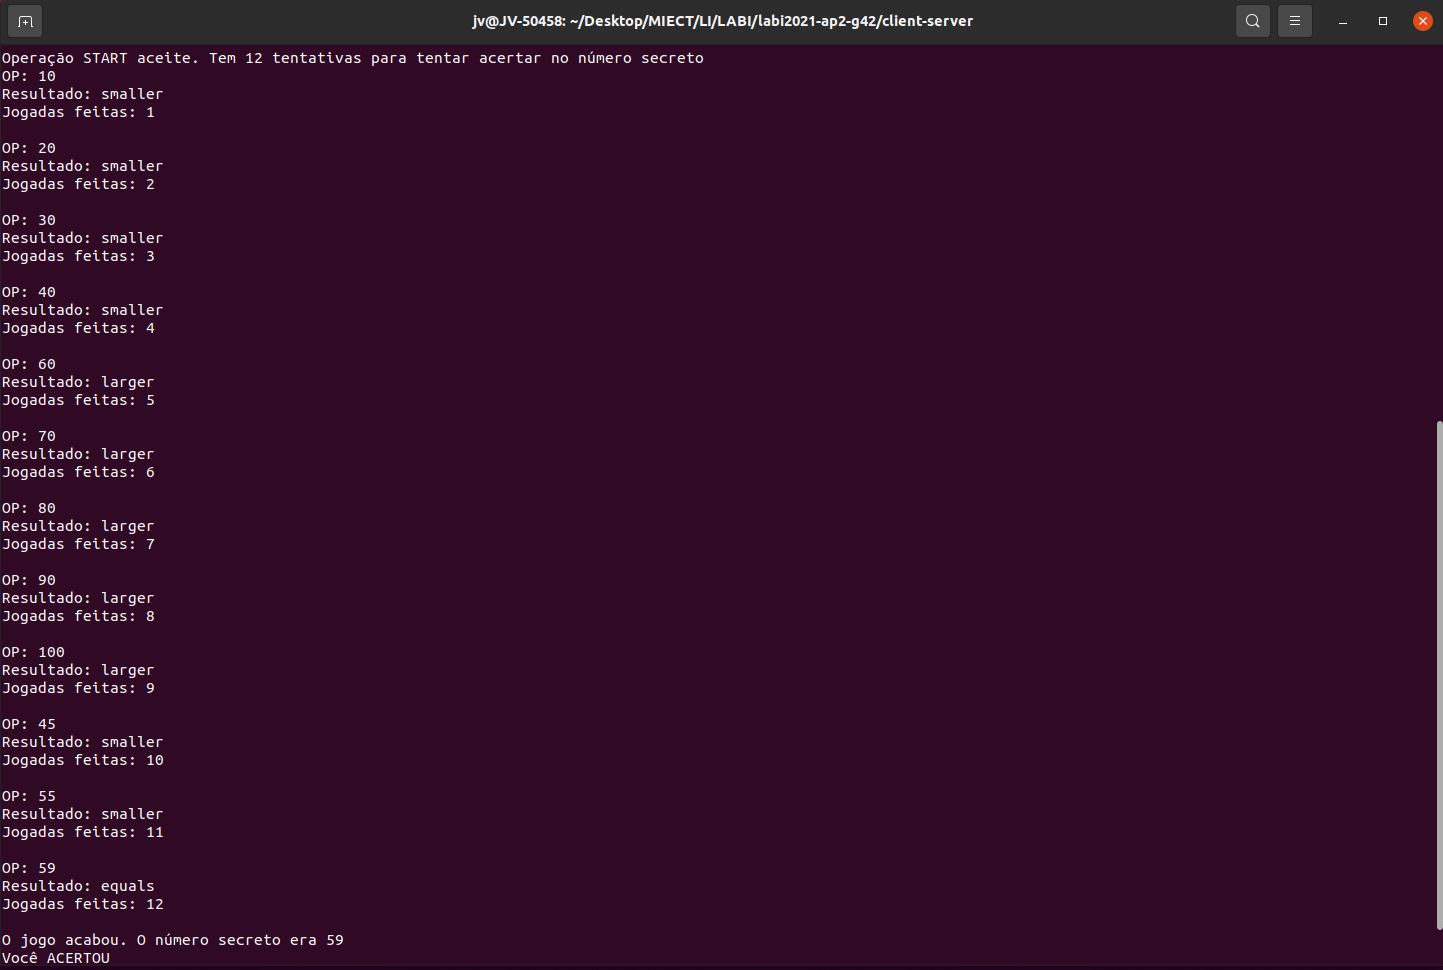
\includegraphics[scale=0.12]{jogo-ganha-ultima}
		\caption{Jogo completo. Cliente ganhou na última.}
		\label{fig:jogo-ganha-ultima}
	\end{subfigure}
	\begin{subfigure}[t]{0.45\textwidth}
		\centering
		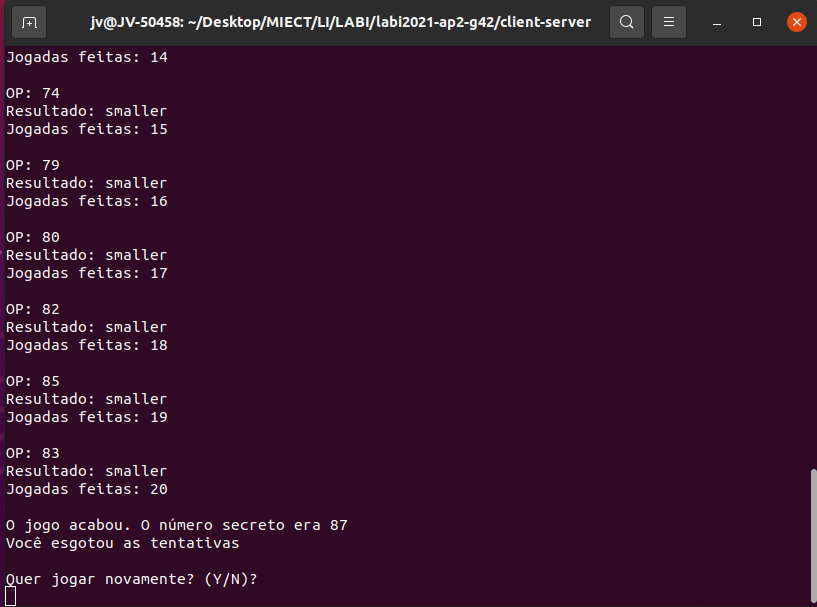
\includegraphics[scale=0.2]{jogo-perde}
		\caption{Jogo completo. Cliente perdeu por esgotar tentativas.}
		\label{fig:jogo-perde}
	\end{subfigure}
	\caption{Simulaçãp de jogo completo. Cliente escolhe se pertende jogar novamente}
	\label{fig:jogo-ganha-perde}
	\flushleft\small\textit{Notas: \\ 1ª Jogada: Cliente adivinha um número inferior ao número secreto (\textit{smaller}). \\ 2ª Jogada: Cliente adivinha um número superior (\textit{larger}). \\ 3ª Jogada: Cliente acerta no número secreto (\textit{equals}). \\ Posteriormente, o cliente escolhe se pretende ou não jogar novamente. }
\end{figure}	

O usuário pode sair do jogo a qualquer momento através do comando \textit{quit}. Nesse caso, a aplicação-Cliente apenas apresenta uma mensagem a informar se o Servidor aceitou a operação e o processo ocorreu sem erros. Qualquer input por parte do usuário que não seja um número ou a operação \textit{quit} gera uma mensagem de erro \textit{Operação Inválida} e nada acontece.

\begin{figure}[H]
	\centering
	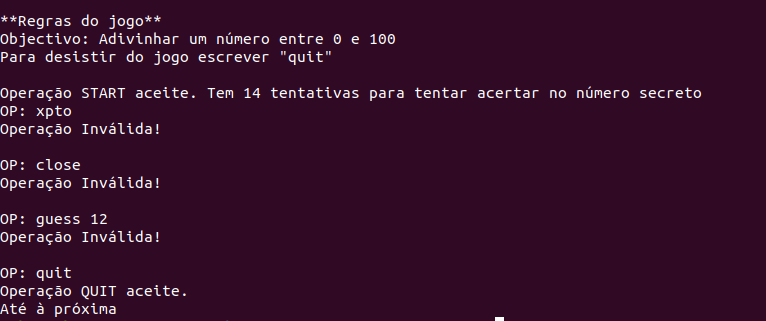
\includegraphics[width=12cm]{func_quit}
	\caption{Funcionamento da operação Quit\\}
	\label{fig:func_quit}
\end{figure} 

\section{Testes do Servidor}

Na secção anterior foi explicado e ilustrado o correcto funcionamento da aplicação-Cliente. Nesta secção são descritos os testes feitos à aplicação-Servidor de forma a confirmar que o código está construído de forma que, caso surjam situações fora do expectável, estas são corrigidas. Para tal foi criado um directório intitulado de \textit{FicheirosTeste} com alguns ficheiros de código que forçam situações de erro e mostram as mensagens enviadas pelo Servidor.

Quando o pedido de inicialização do jogo é aceite pelo Servidor este acrescenta à lista de jogadores activos os dados do Cliente que efectuou o pedido.
Sempre que o Servidor recebe uma mensagem/operação de um Cliente a primeira coisa que deve ser feita é confirmar que esse Cliente está a jogar, verificando a lista de jogadores activos. Se o Sevidor recebe uma mensagem de um Cliente não activo, o Servidor deve enviar uma mensagem de erro.
É importante referir que o Cliente está implementado de forma que termine imediatamente sempre que receba uma mensagem de erro. Esta funcionalidade é expressamente pedida no enunciado do trabalho. 

\begin{figure}[H]
	\centering
	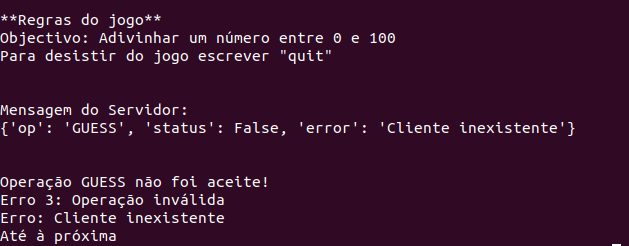
\includegraphics[width=12cm]{test1}
	\caption{Operação \textit{Guess} enviada por um Cliente não activo\\}
	\label{fig:test1}
\end{figure} 

\begin{figure}[H]
	\centering
	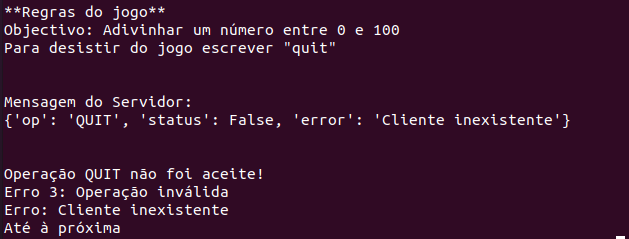
\includegraphics[width=12cm]{test2}
	\caption{Operação \textit{Quit} enviada por um Cliente não activo\\}
	\label{fig:test2}
\end{figure} 

\begin{figure}[H]
	\centering
	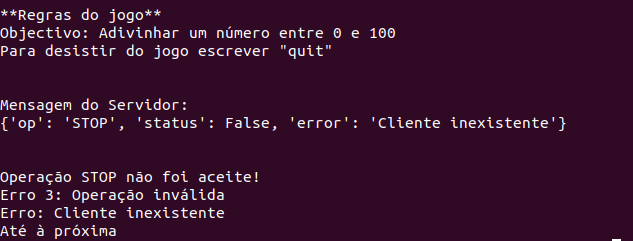
\includegraphics[width=12cm]{test3}
	\caption{Operação \textit{Stop} enviada por um Cliente não activo\\}
	\label{fig:test3}
\end{figure} 

Na operação \textit{Stop} o Servidor faz uma verificação adicional para se certificar que o número de tentativas jogadas reportado pelo Cliente é igual ao número de tentativas registadas pelo próprio Servidor. Se houver alguma discrepância entre os dois registos o Servidor envia uma mensagem de erro.

\begin{figure}[H]
	\centering
	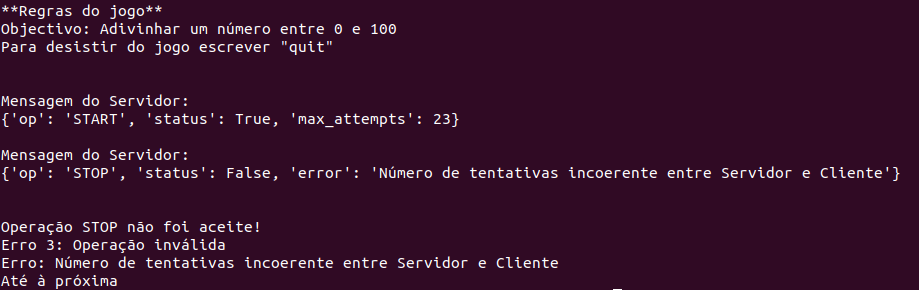
\includegraphics[width=12cm]{test4}
	\caption{Incoerência entre tentativas registadas pelo Servidor e Cliente\\}
	\label{fig:test4}
\end{figure} 

Se por alguma razão o Servidor receber uma operação fora dos parâmetros possíveis, este deve enviar uma mensagem de erro informando que a operação é inexistente.

\begin{figure}[H]
	\centering
	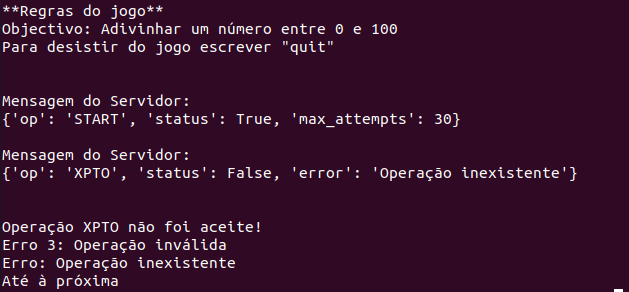
\includegraphics[width=12cm]{test5}
	\caption{Cliente envia operação inexistente ao Servidor\\}
	\label{fig:test5}
\end{figure} 

Ao longo do desenvolvimento deste projecto foram encontrados e corrigidos vários erros, no entanto, para o âmbito deste relatório, decidiu-se não os explorar exaustivamente devido à sua pouca relevância. A maioria destes erros estavam relacionados com as funções \textit{find-client}, \textit{clean-client}, \textit{create-file}, \textit{update-file} e variáveis globais.

Também se considerou importante referir que aplicação começou por ser implementada duma maneira diferente do proposto por algum lapso de interpretação do enunciado, sendo que o código desenvolvido nessa fase encontra-se na pasta \textit{Alt-ServClient}. Essa versão da aplicação, apesar de não ter sido terminada, está funcional e pode ser útil para futuros projectos uma vez que contém vários mecanismos adicionais à versão final para manter a sua robustez.


\section{Analise de Resultados}
\label{sec.analise-resultados}
Como se pode verificar nas secções anteriores, o programa aparenta funcionar correctamente e de acordo com as especificações pedidas no enunciado. As funcionalidades adicionadas pelos autores também aparentam funcionar de maneira correcta, complementando o projecto. \\
Todos os bugs encontrados foram corrigidos, e todas a situações de erro previstas foram tratadas, tornando assim o programa o mais robusto possível dadas as normas do enunciado e o prazo de entrega.\\

%
%%%%%%%%%%%%%%%%%%%%%%%%%%%%%%%%%%%%%%%%%%%%%%%%%%%%%%%%%
%%%%%CAPÍTULO 3: CONCLUSÃO
%
\chapter{Conclusão:}
\label{chap.conclusão}
\lhead{Conclusão}

Dados os resultados obtidos podemos concluir que a elaboração deste projecto foi bem sucedida. Não só foi possível implementar o que era pedido, como ainda desenvolvemos funcionalidades extra que consideramos complementarem o projecto. \\
Este projecto foi bastante útil para desenvolver competências de programação Python, tanto em termos de domínio de linguagem, como de estruturação de código. Além disso este trabalho abordou uma variedade doutras matérias nomeadamente programação de Sockets, documentos JSON e CSV, criptografia e GIT.\\
Finalizamos o trabalho com a noção de que, apesar do seu sucesso, tendo um periodo mais alargado seria possível expandir consideravelmente o projecto. \\

%
%%%%%%%%%%%%%%%%%%%%%%%%%%%%%%%%%%%%%%%%%%%%%%%%%%%%%%%%%
%%%%%CONTRIBUIÇÕES DE AUTORES:
% 
\chapter*{Contribuições dos Autores}

\begin{table}[H]
    \centering
    \caption{Contribuições dos Autores.}
    \begin{tabular}{|c|c|c|c|}\hline
        Contribuição & Rui Machado & João Vieira  \\ 
        \hline
	    Produção de Relatório & 50~\% & 50~\%    \\
	    Desenvolvimento de Código & 80~\% & 20~\%  \\
	    Implementação de Segurança & 60~\% & 40~\% \\ 
		Testes e Depuração & 60~\% & 40~\% \\   
    \hline
    \end{tabular}
    \label{tab.contribuições}
\end{table}	

%
%%%%%%%%%%%%%%%%%%%%%%%%%%%%%%%%%%%%%%%%%%%%%%%%%%%%%%%%%
%%%%%BIBLIOGRAFIA:
%
\begin{thebibliography}{9}

\bibitem{thinkpython} 
Allen Downey
\textit{Think Python - How to Think Like a Computer Scientist}. |
Green Tea Press, 2nd Edition, Version 2.4.0, 2015

\bibitem{pycryptome}
PyCryptodome documentation. |
\text{ pycryptodome.readthedocs.io, acedido 18/05/2021.}

\bibitem{Wikipedia}
Wikipédia: Enciclopédia livre. |
\text{ pt.wikipedia.org, acedido 19/05/2021.}

\bibitem{serverfault}
ServerFault Website. |
\text{ serverfault.com, acedido 22/05/2021.}

\bibitem{iana}
Internet Assigned Numbers Authority. |
\text{ www.iana.org, acedido 22/05/2021.}


\end{thebibliography}
\end{document}
